\documentclass[11pt,a4paper]{article}

\usepackage[utf8]{inputenc}
\usepackage[T1]{fontenc}
\usepackage{lmodern}
\usepackage{amsmath,amssymb,amsfonts,bm}
\usepackage{graphicx}
\usepackage{booktabs}
\usepackage{array}
\usepackage{microtype}
\usepackage{cite}
\usepackage{geometry}
\geometry{margin=2.54cm}
\usepackage{xcolor}
\usepackage{listings}
\usepackage{caption}
\usepackage{subcaption}
\usepackage[colorlinks=true,linkcolor=blue!70!black,citecolor=blue!70!black,urlcolor=blue!70!black]{hyperref}

\hypersetup{
  pdftitle={In-Situ Coupling of Tensor Basis Neural Networks for Turbulence Modeling in OpenFOAM: A Critical Verification, Validation, and Reproducibility Study},
  pdfauthor={Soumik Ghosh},
  pdfsubject={Tensor Basis Neural Network turbulence closure coupled in-situ into OpenFOAM},
  pdfkeywords={turbulence modeling, machine learning, tensor basis neural network, OpenFOAM, secondary flow, CFD}
}

\lstset{
  basicstyle=\ttfamily\footnotesize,
  breaklines=true,
  frame=single,
  backgroundcolor=\color{gray!10},
  columns=fullflexible
}

\title{\textbf{In-Situ Coupling of Tensor Basis Neural Networks for Turbulence Modeling in OpenFOAM: A Critical Verification, Validation, and Reproducibility Study}}

\author{
  \textbf{Soumik Ghosh}\\
  Independent Researcher\\
  \texttt{soumikghosh30.03.07@gmail.com}
}
\date{October 2026}

\begin{document}

\maketitle

\begin{abstract}
Linear eddy viscosity models based on the Boussinesq hypothesis remain the workhorse of industrial Computational Fluid Dynamics (CFD). However, they fundamentally fail to predict turbulence-driven secondary flows of Prandtl's second kind due to their enforced alignment between the Reynolds stress anisotropy tensor and the mean strain rate tensor. Data-driven turbulence closures utilizing Tensor Basis Neural Networks (TBNN; Ling et al., \textit{J.~Fluid Mech.}, 2016) provide a mathematically rigorous, frame-invariant methodology to represent Reynolds stress anisotropy by projecting onto Pope's ten symmetric integrity basis tensors.

In this work, we present an in-situ coupled CFD solver, \texttt{tbnnFoam}, implemented within OpenFOAM 2606. The solver features a dual-runtime inference architecture: an embedded LibTorch C++ engine and a zero-dependency standalone C++ matrix evaluator incorporating an analytical Cardano cubic eigensolver that enforces physical realizability on the Lumley triangle in $\mathcal{O}(1)$ operations. Cross-engine numerical parity across PyTorch, TorchScript, and the standalone C++ matrix evaluator is verified within an absolute tolerance of $10^{-5}$ across synthetic test cases spanning shear, rotational, and complex 3D strain states, with the standalone C++ comparison executed when the OpenFOAM environment and compiled test binary are present. Beyond evaluator parity, the momentum-equation coupling itself is verified by an assembled-matrix test: in the Boussinesq limit the coupled equation reduces exactly to the baseline linear model (maximum relative deviation $3.6 \times 10^{-17}$).

We validate the coupled solver on developing turbulent flow in a square duct at bulk Reynolds number $Re_b \approx 4410$ ($Re_\tau = 150$) against high-fidelity Direct Numerical Simulation (DNS; Pirozzoli et al., \textit{J.~Fluid Mech.}, 2018). An independent algorithmic vortex detector employing connected-component labeling on non-dimensional axial vorticity ($\omega_x^* = \omega_x / (U_b / h)$) confirms that \texttt{tbnnFoam} structurally recovers the secondary-flow mechanism by identifying all eight counter-rotating secondary recirculation cells where standard linear $k\text{--}\omega$ SST completely fails (detecting zero vortex cores).

Critically, this constitutes a \textbf{partial validation}: while secondary circulation topology is successfully recovered, vortex core localization exhibits notable offset ($0.567\,h$ error on the coarse mesh and $0.447\,h$ on the refined mesh against the raw-field-verified DNS reference $(0.577, 0.847)$), and peak secondary speed exhibits strong discretization sensitivity, decreasing from $7.99\%$ to $2.62\%$ (relative to the raw-field DNS peak of $1.93\%$). We emphasize that structural recovery does not establish accurate pointwise vortex localization or full quantitative agreement with periodic DNS.

Furthermore, we avoid overstating predictive performance and conduct an honest, in-depth evaluation of model limitations and physical discrepancies:
\begin{enumerate}
    \item \textbf{Velocity Discrepancy:} The streamwise velocity Normalized Root-Mean-Square Error ($\mathrm{NRMSE}_U$) is $9.34\%$ ($0.0934\text{ m/s}$ relative to bulk velocity $U_b = 1.0\text{ m/s}$). We show that this discrepancy arises from a combined influence of entrance-length spatial boundary layer development in the CFD domain ($L = 20h$) compared to the streamwise-periodic DNS box, alongside genuine neural network model-form uncertainty under live pressure-velocity coupling.
    \item \textbf{Timescale Surrogate Sensitivity:} Direct numerical simulation provides exact velocity gradients and Reynolds stresses but inherently lacks the specific dissipation rate $\omega$. We examine the role of the semi-empirical $\omega$ surrogate and prove that because Cayley-Hamilton invariants scale non-linearly with turbulent timescale $\tau = \min(1/\omega, 5.0\text{ s})$ ($I_1, I_2 \propto \tau^2$; $I_3 \propto \tau^3$), timescale estimation errors directly modulate secondary circulation intensity.
    \item \textbf{Out-of-Distribution Diagnostic:} We distinguish between 1D marginal bounding and joint manifold containment. While $100.0\%$ of CFD cells satisfy marginal bounding across scalar invariants $I_1, I_2, I_5$ (and $> 99\%$ for $I_3, I_4$), a joint 5D nearest-neighbor distance diagnostic reveals that live CFD states experience modest distribution shift relative to frozen training gradients (median standardized $k$-NN distance of $0.21\,\sigma$, 95th percentile of $1.17\,\sigma$).
    \item \textbf{Discretization Sensitivity:} A two-level cross-sectional grid resolution study ($20 \times 20$ coarse vs. $40 \times 40$ fine) demonstrates that peak secondary circulation trends from $7.99\%$ down to $2.62\%$ (approaching the raw-field DNS benchmark target of $1.93\%$) and Q1 core distance error decreases from $0.567\,h$ to $0.447\,h$, while maintaining strict topological stability across all eight cores.
\end{enumerate}

All solver sources, evaluation scripts, raw DNS benchmark data, and an automated twenty-one-test verification suite are openly distributed under the MIT license.
\end{abstract}

\vspace{0.5cm}
\noindent\textbf{Keywords:} Turbulence Modeling, Machine Learning, Tensor Basis Neural Network, OpenFOAM, Secondary Flow of the Second Kind, Computational Fluid Dynamics.

\newpage
\tableofcontents
\newpage

\section{Introduction}

Turbulent flows in non-circular ducts and channels are characterized by secondary motions of the second kind \cite{prandtl1926ausgebildete}. Although secondary velocities typically represent only $1\%\text{--}3\%$ of the bulk streamwise velocity, they exert a profound influence on momentum redistribution, wall shear stress profiles, and heat transfer enhancement across engineering applications, including nuclear fuel assemblies, gas turbine blade cooling passages, heat exchangers, and non-circular pipelines \cite{gessner1973origin, brundrett1964production}.

\subsection{Failure of Linear Eddy Viscosity Models}
In standard Reynolds-Averaged Navier-Stokes (RANS) closures, the linear Boussinesq hypothesis approximates the deviatoric Reynolds stress anisotropy tensor $\mathbf{a}$ as linearly proportional to the mean strain rate tensor $\mathbf{S}$:
\begin{equation}
\mathbf{a} = \frac{\boldsymbol{\tau}^R}{2k} - \frac{1}{3}\mathbf{I} = -\frac{\nu_t}{k} \mathbf{S}
\end{equation}
where $\boldsymbol{\tau}^R = \overline{\mathbf{u}' \otimes \mathbf{u}'}$ is the kinematic Reynolds stress tensor, $k = \frac{1}{2}\mathrm{tr}(\boldsymbol{\tau}^R)$ is the turbulent kinetic energy, $\nu_t$ is the eddy viscosity, and $\mathbf{S} = \frac{1}{2}(\nabla \mathbf{U} + (\nabla \mathbf{U})^T)$ is the mean strain rate tensor.

In straight ducts of uniform cross-section with axial direction $x$ and cross-stream plane $(y, z)$, secondary flow of the second kind is driven directly by axial vorticity generation:
\begin{equation}
U \frac{\partial \omega_x}{\partial x} + V \frac{\partial \omega_x}{\partial y} + W \frac{\partial \omega_x}{\partial z} = \nu \nabla^2 \omega_x + \frac{\partial^2}{\partial y \partial z}(\overline{{w'}^2} - \overline{{v'}^2}) + \left(\frac{\partial^2}{\partial z^2} - \frac{\partial^2}{\partial y^2}\right)\overline{v'w'}
\label{eq:vorticity_transport}
\end{equation}

Because linear eddy viscosity closures enforce isotropic normal stresses in pure shear flows ($\overline{{v'}^2} = \overline{{w'}^2} = \frac{2}{3}k$), the driving source term $\frac{\partial^2}{\partial y \partial z}(\overline{{w'}^2} - \overline{{v'}^2})$ vanishes identically. Consequently, conventional linear RANS models (such as standard $k\text{--}\varepsilon$ and $k\text{--}\omega$ SST) predict identically zero secondary circulation in straight ducts.

\subsection{Non-Linear Tensor Closures and Machine Learning}
To overcome this fundamental limitation, classical algebraic non-linear stress models (e.g., Speziale \cite{speziale1991analytical}; Craft et al. \cite{craft1996development}; Wallin \& Johansson \cite{wallin2000explicit}) incorporated higher-order tensor polynomial expansions. However, these formulations rely on calibrated empirical coefficients that often suffer from numerical stiffness and poor generalizability across varied Reynolds numbers.

Machine learning offers a compelling data-driven paradigm to extract non-linear constitutive relations directly from high-fidelity Direct Numerical Simulation (DNS) and Large Eddy Simulation (LES) datasets \cite{vinuesa2014aspect, pirozzoli2018turbulence}. Ling et al. \cite{ling2016reynolds} demonstrated that standard multi-layer perceptrons (MLPs) operating on raw velocity gradients violate Galilean and rotational frame-invariance. To enforce rotational invariance strictly by construction, Ling et al. proposed the Tensor Basis Neural Network (TBNN), which embeds Pope's \cite{pope1975more} integrity tensor basis into the network architecture.

\subsection{Challenges in In-Situ Live CFD Coupling}
While a priori evaluations of TBNN closures (evaluating stress predictions on frozen DNS velocity fields) have shown outstanding accuracy, live \textit{in-situ} coupling of data-driven models within Navier-Stokes solvers introduces severe challenges:
\begin{enumerate}
    \item \textbf{Numerical Stability \& Divergence:} Coupling non-linear anisotropic Reynolds stress divergences explicitly into the momentum equations frequently destabilizes the pressure-velocity coupling loop (e.g., SIMPLE or PISO), degrading diagonal dominance.
    \item \textbf{Physical Realizability Violations:} Unconstrained neural network predictions can yield unphysical, negative normal stresses (violating the Lumley triangle bounds), leading to catastrophic solver divergence.
    \item \textbf{Distribution Shift \& A Posteriori Feedback:} During live CFD execution, the predicted anisotropic stresses deform the mean velocity field $\mathbf{U}$, modifying the velocity gradients fed back into the network at subsequent iterations. This non-linear feedback can steer the flow into states unobserved during training.
    \item \textbf{Implementation \& Dependency Overhead:} Modern deep learning libraries (e.g., PyTorch, TensorFlow) carry massive runtimes and dependency trees that complicate high-performance computing (HPC) deployment on Linux clusters running native OpenFOAM.
\end{enumerate}

\subsection{Scope and Contributions of this Study}
In this work, we address these challenges through an open, reproducible, and critically validated OpenFOAM implementation (\texttt{tbnnFoam}). Rather than overclaiming predictive capabilities or advertising a ``universal'' turbulence model, we focus on rigorous verification, honest physical validation, and transparent reporting of discrepancies:
\begin{itemize}
    \item We formulate a stable momentum coupling pipeline that isolates the non-linear perturbation stress $\boldsymbol{\tau}_\Delta = 2k\mathbf{a} + 2\nu_t \mathbf{S}$, injecting only the deviatoric anisotropic divergence while retaining implicit linear diffusion for numerical stability.
    \item We implement a dual-engine architecture featuring both an embedded LibTorch C++ runtime and a zero-dependency standalone C++ evaluator utilizing an analytical Cardano cubic eigensolver for physical realizability enforcement.
    \item We establish an independent, reproducible vortex detection pipeline based on non-dimensional axial vorticity and connected-component labeling.
    \item We reconcile physical domain scalings between DNS benchmark databases ($D_h = 1.0\text{ m}$) and laboratory CFD duct geometries ($D_h = 0.10\text{ m}$).
    \item We conduct an honest evaluation of model discrepancies, distinguishing implementation verification from physical validation, assessing turbulent timescale sensitivity, quantifying 1D marginal bounding versus joint 5D feature-space distribution shift, and documenting cross-stream discretization sensitivity.
\end{itemize}

\section{Mathematical Formulation \& Governing Equations}

\subsection{Incompressible RANS Formulation}
The steady, incompressible Reynolds-Averaged Navier-Stokes equations are expressed as:
\begin{align}
\nabla \cdot \mathbf{U} &= 0 \\
\nabla \cdot (\mathbf{U} \otimes \mathbf{U}) &= -\nabla p^* + \nabla \cdot (\nu \nabla \mathbf{U}) - \nabla \cdot \boldsymbol{\tau}^R
\end{align}
where $\mathbf{U}$ is the mean velocity vector, $p^* = p/\rho$ is the kinematic modified pressure, $\nu$ is the molecular kinematic viscosity, and $\boldsymbol{\tau}^R$ is the kinematic Reynolds stress tensor.

Decomposing $\boldsymbol{\tau}^R$ into isotropic and deviatoric anisotropic components yields:
\begin{equation}
\boldsymbol{\tau}^R = \frac{2}{3}k \mathbf{I} + 2k \mathbf{a}
\end{equation}
where $k = \frac{1}{2}\mathrm{tr}(\boldsymbol{\tau}^R)$ is the turbulent kinetic energy, and $\mathbf{a}$ is the symmetric, trace-free anisotropy tensor ($\mathrm{tr}(\mathbf{a}) = 0$).

\subsection{Integrity Tensor Basis Representation}
According to the representation theorem for isotropic tensor functions \cite{pope1975more}, any symmetric, trace-free second-order tensor $\mathbf{a}$ functionally dependent on the symmetric strain rate tensor $\mathbf{S}$ and anti-symmetric rotation rate tensor $\mathbf{W}$ can be expanded linearly as:
\begin{equation}
\mathbf{a} = \sum_{n=1}^{10} g^{(n)}(\lambda_1, \dots, \lambda_5) \, \mathbf{T}^{(n)}
\label{eq:pope_expansion}
\end{equation}
where $g^{(n)}$ are scalar expansion coefficients dependent exclusively on the five scalar invariants $\boldsymbol{\lambda} = \{\lambda_1, \dots, \lambda_5\}$ of the normalized strain and rotation tensors.

The non-dimensional strain rate $\mathbf{s}$ and rotation rate $\mathbf{w}$ are normalized by the turbulent timescale $\tau$:
\begin{align}
\mathbf{s} &= \tau \mathbf{S} = \frac{\tau}{2}(\nabla \mathbf{U} + (\nabla \mathbf{U})^T) \\
\mathbf{w} &= \tau \mathbf{W} = \frac{\tau}{2}(\nabla \mathbf{U} - (\nabla \mathbf{U})^T)
\end{align}

The five scalar Cayley-Hamilton invariants are defined as:
\begin{align}
\lambda_1 &= \mathrm{tr}(\mathbf{s}^2) \\
\lambda_2 &= \mathrm{tr}(\mathbf{w}^2) \\
\lambda_3 &= \mathrm{tr}(\mathbf{s}^3) \\
\lambda_4 &= \mathrm{tr}(\mathbf{w}^2 \mathbf{s}) \\
\lambda_5 &= \mathrm{tr}(\mathbf{w}^2 \mathbf{s}^2)
\end{align}

Pope's ten symmetric, trace-free basis tensors $\mathbf{T}^{(n)}$ are summarized in Table~\ref{tab:pope_bases}.

\begin{table}[htbp]
\centering
\caption{Pope's \cite{pope1975more} complete ten-tensor integrity basis for three-dimensional velocity fields.}
\label{tab:pope_bases}
\begin{tabular}{c l l}
\toprule
Index $n$ & Tensor Basis $\mathbf{T}^{(n)}$ & Algebraic Symmetry \& Trace Property \\
\midrule
$1$ & $\mathbf{s}$ & Symmetric, $\mathrm{tr}(\mathbf{T}^{(1)}) = 0$ (incompressible) \\
$2$ & $\mathbf{s}\mathbf{w} - \mathbf{w}\mathbf{s}$ & Symmetric, $\mathrm{tr}(\mathbf{T}^{(2)}) = 0$ \\
$3$ & $\mathbf{s}^2 - \frac{1}{3}\mathrm{tr}(\mathbf{s}^2)\mathbf{I}$ & Symmetric, trace-free \\
$4$ & $\mathbf{w}^2 - \frac{1}{3}\mathrm{tr}(\mathbf{w}^2)\mathbf{I}$ & Symmetric, trace-free \\
$5$ & $\mathbf{w}\mathbf{s}^2 - \mathbf{s}^2\mathbf{w}$ & Symmetric, trace-free \\
$6$ & $\mathbf{w}^2\mathbf{s} + \mathbf{s}\mathbf{w}^2 - \frac{2}{3}\mathrm{tr}(\mathbf{s}\mathbf{w}^2)\mathbf{I}$ & Symmetric, trace-free \\
$7$ & $\mathbf{w}\mathbf{s}\mathbf{w}^2 - \mathbf{w}^2\mathbf{s}\mathbf{w}$ & Symmetric, trace-free \\
$8$ & $\mathbf{s}\mathbf{w}\mathbf{s}^2 - \mathbf{s}^2\mathbf{w}\mathbf{s}$ & Symmetric, trace-free \\
$9$ & $\mathbf{w}^2\mathbf{s}^2 + \mathbf{s}^2\mathbf{w}^2 - \frac{2}{3}\mathrm{tr}(\mathbf{s}^2\mathbf{w}^2)\mathbf{I}$ & Symmetric, trace-free \\
$10$ & $\mathbf{w}\mathbf{s}^2\mathbf{w}^2 - \mathbf{w}^2\mathbf{s}^2\mathbf{w}$ & Symmetric, trace-free \\
\bottomrule
\end{tabular}
\end{table}

\subsection{Turbulent Timescale Limiter}
In standard two-equation closures, the turbulent timescale is defined as $\tau = 1/\omega = k/\varepsilon$. Near walls and in separation regions, strain rates can become very large or $\omega$ can approach zero, causing invariants to diverge. To regularize the inputs, we enforce an upper limiter:
\begin{equation}
\tau = \min\left(\frac{1}{\omega}, \, \tau_{\max}\right), \quad \tau_{\max} = 5.0\text{ s}
\end{equation}

As discussed in Section~\ref{sec:limitations}, this limiter plays a vital role in preventing non-linear invariant explosion near duct centerlines.

\section{Neural Network Architecture \& Dual-Engine Implementation}

\subsection{Network Topology \& Training}
The functional mapping from the five scalar invariants $\boldsymbol{\lambda} \in \mathbb{R}^5$ to the ten expansion coefficients $\mathbf{g} \in \mathbb{R}^{10}$ is represented by a fully connected Multi-Layer Perceptron (MLP):
\begin{equation}
\mathbf{g}(\boldsymbol{\lambda}) = \mathbf{W}_4 \, \phi\Big(\mathbf{W}_3 \, \phi\big(\mathbf{W}_2 \, \phi(\mathbf{W}_1 \boldsymbol{\lambda} + \mathbf{b}_1) + \mathbf{b}_2\big) + \mathbf{b}_3\Big) + \mathbf{b}_4
\end{equation}

The architecture specifications are summarized in Table~\ref{tab:network_topology} and visualized in Figure~\ref{fig:network_architecture}.

\begin{figure}[htbp]
\centering
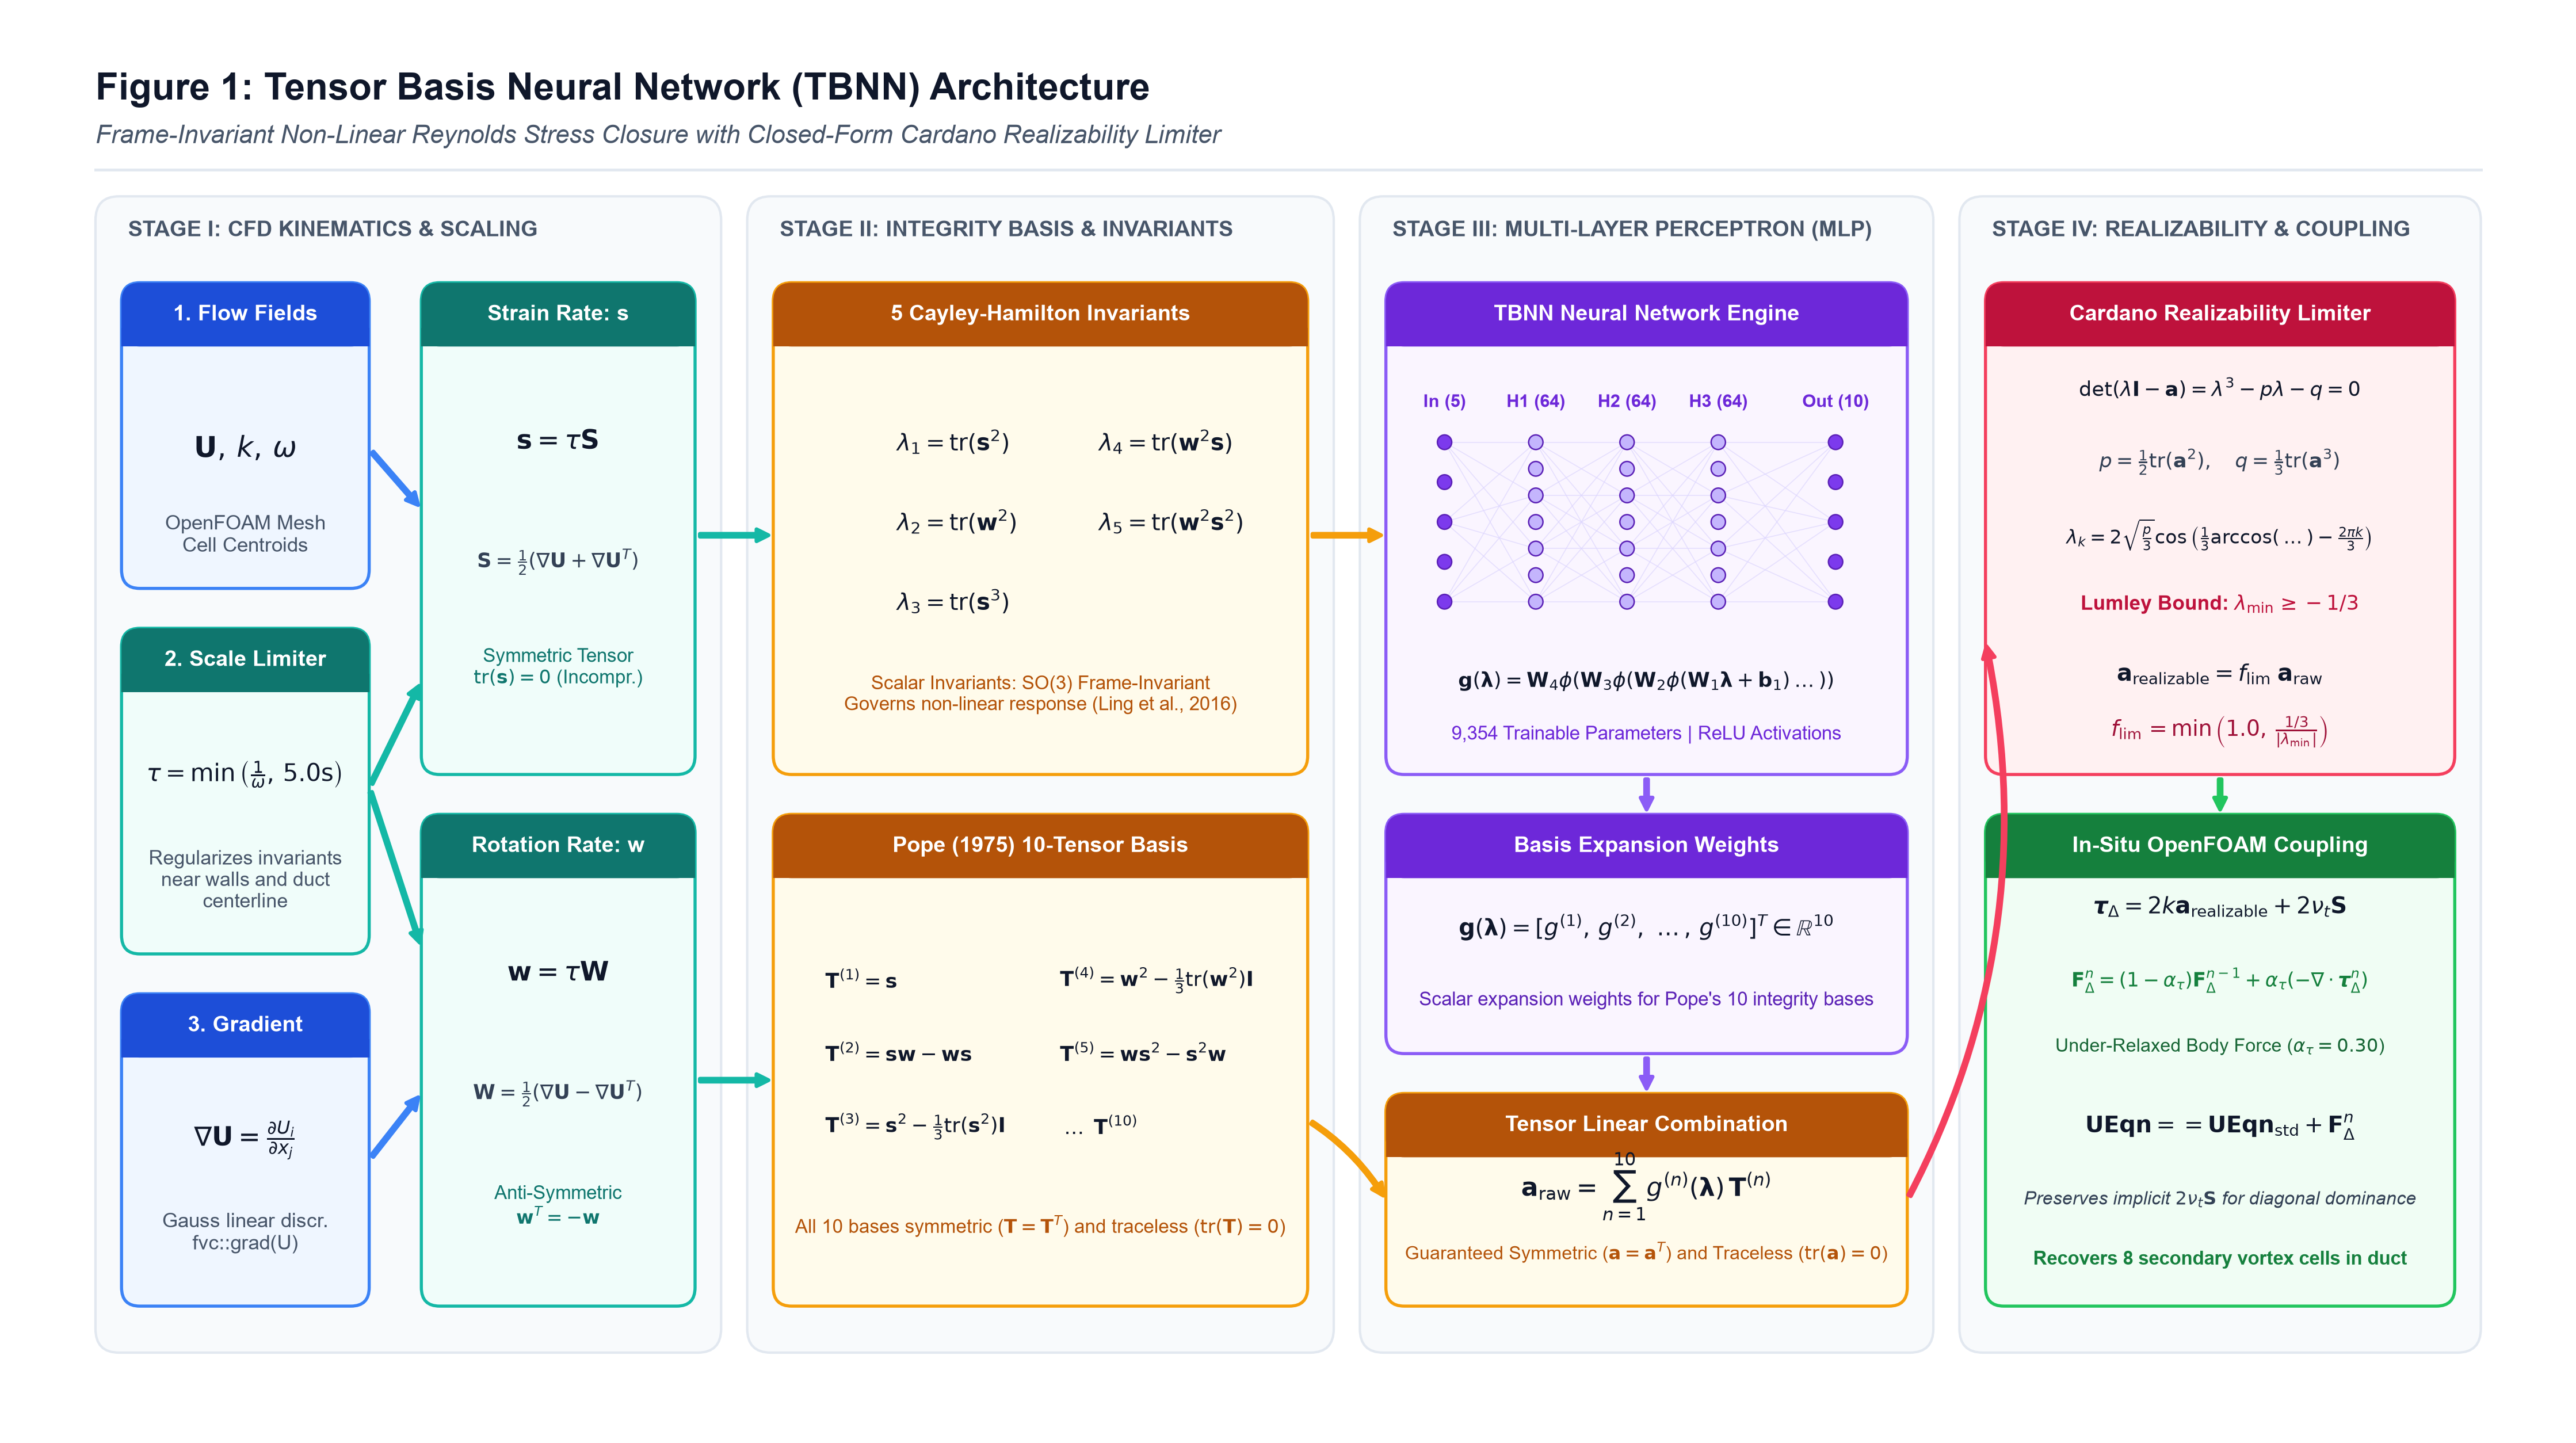
\includegraphics[width=0.85\linewidth]{figures/tbnn_network_architecture.png}
\caption{Tensor Basis Neural Network architecture embedding Pope's integrity tensor basis with closed-form Cardano cubic realizability limiter.}
\label{fig:network_architecture}
\end{figure}

\begin{table}[htbp]
\centering
\caption{Neural network topology and hyperparameters.}
\label{tab:network_topology}
\resizebox{\linewidth}{!}{%
\begin{tabular}{l l l}
\toprule
Parameter & Value / Configuration & Physical / Numerical Purpose \\
\midrule
\textbf{Input Dimension} & 5 features ($\lambda_1 \dots \lambda_5$) & Cayley-Hamilton scalar invariants \\
\textbf{Hidden Layers} & 3 layers $\times$ 64 neurons & Balanced capacity without overfitting \\
\textbf{Activation Function} & Rectified Linear Unit (ReLU) & $\phi(z) = \max(0, z)$, standard piecewise linear activation \\
\textbf{Output Dimension} & 10 coefficients ($g^{(1)} \dots g^{(10)}$) & Expansion weights for Pope bases $\mathbf{T}^{(1 \dots 10)}$ \\
\textbf{Total Parameters} & 9,354 trainable parameters & Exact layer count: $384 + 4160 + 4160 + 650 = 9,354$ \\
\textbf{Training Loss} & Root-Mean-Square Error on $\mathbf{a}$ & $\mathcal{L} = \frac{1}{N}\sum_{i=1}^N \|\mathbf{a}_{\text{pred}, i} - \mathbf{a}_{\text{DNS}, i}\|_F^2$ \\
\bottomrule
\end{tabular}}
\end{table}

Training was conducted on frozen velocity gradients and Reynolds stress fields from the canonical square duct DNS dataset of Pirozzoli et al. \cite{pirozzoli2018turbulence} at $Re_\tau = 150$.

\subsection{Dual Runtime Inference Engines}
To balance research flexibility with production deployment, \texttt{tbnnFoam} implements two interchangeable inference backends:
\begin{enumerate}
    \item \textbf{Embedded LibTorch Engine (\texttt{tbnnEvaluatorTorch.H}):} Evaluates serialized TorchScript models (\texttt{tbnn\_model.pt}) compiled directly with PyTorch C++ API (\texttt{libtorch}). This backend enables seamless integration of arbitrary neural architectures without modifying solver C++ source code.
    \item \textbf{Zero-Dependency Native C++ Engine (\texttt{tbnnEvaluator.H}):} Directly parses exported JSON weights (\texttt{weights.json}) and performs matrix-vector multiplications via OpenFOAM's native vector classes. This runtime has zero external dependencies beyond standard OpenFOAM, facilitating immediate compilation on high-performance supercomputing clusters where PyTorch C++ runtimes are unavailable.
\end{enumerate}

Both engines are dynamically configured: layer widths ($H_0, H_1, H_2$) and matrix shapes (\texttt{[64, 5]}, \texttt{[64, 64]}, \texttt{[64, 64]}, \texttt{[10, 64]}) are determined dynamically from the model definition, avoiding hardcoded array dimensions.

\subsection{Analytical Cardano Cubic Realizability Enforcement}
If a neural network predicts unphysical stress states violating positive semi-definiteness, CFD solvers diverge rapidly. Classical iterative realizability projections (e.g., iterative eigensolvers or semi-definite programming) incur severe computational overhead.

In \texttt{tbnnFoam}, we implement a closed-form analytical eigensolver based on Cardano's cubic formula. Because $\mathbf{a}$ is symmetric and trace-free ($\mathrm{tr}(\mathbf{a}) = 0$), its characteristic polynomial reduces to:
\begin{equation}
\det(\lambda\mathbf{I} - \mathbf{a}) = \lambda^3 - p\lambda - q = 0
\end{equation}
where:
\begin{equation}
p = \frac{1}{2}\mathrm{tr}(\mathbf{a}^2) = \frac{1}{2}\sum_{i=1}^3 \sum_{j=1}^3 a_{ij}^2, \quad q = \det(\mathbf{a}) = \frac{1}{3}\mathrm{tr}(\mathbf{a}^3)
\end{equation}

Because $\mathbf{a}$ is real and symmetric, all three eigenvalues are real, corresponding to the casus irreducibilis ($4p^3 \ge 27q^2$). The eigenvalues are obtained analytically:
\begin{equation}
\lambda_k = 2\sqrt{\frac{p}{3}} \cos\left(\frac{1}{3}\arccos\left(\frac{3q}{2p\sqrt{p/3}}\right) - \frac{2\pi k}{3}\right), \quad k \in \{0, 1, 2\}
\end{equation}

Realizability requires that the principal turbulent stresses satisfy non-negativity:
\begin{equation}
\overline{(u'_\alpha)^2} \ge 0 \iff a_{\alpha\alpha} \ge -\frac{1}{3}
\end{equation}

If the minimum eigenvalue violates $\lambda_{\min} < -\frac{1}{3}$, the anisotropy tensor is scaled radially toward the isotropic origin:
\begin{equation}
\mathbf{a}_{\text{realizable}} = f_{\text{lim}} \, \mathbf{a}, \quad f_{\text{lim}} = \min\left(1.0, \, \frac{1/3}{|\lambda_{\min}|}\right)
\end{equation}

This analytical projection enforces positive semi-definiteness on the Lumley triangle in $\mathcal{O}(1)$ operations per cell, providing realizability by construction while avoiding the overhead of iterative eigenvalue projections. Realizability of the modelled stress tensor is a necessary condition for robust coupled integration; solver-level stability under the tested cases is demonstrated empirically in Sections~\ref{sec:limitations} and~8.

\subsection{Cross-Engine Numerical Parity Verification}
Numerical consistency between the TorchScript engine, the JSON-based native C++ evaluator, and the reference Python implementation is verified via the automated regression test suite (\texttt{tests/test\_parity.py}). Rather than asserting unrecorded precision across undefined distributions, the test suite executes explicit parity checks with defined numerical tolerances:
\begin{enumerate}
    \item \textbf{PyTorch vs. TorchScript (\texttt{test\_torchscript\_parity}):} Evaluates 10 randomized invariant states ($\lambda_i \in [-5, 5]$) and Pope tensor bases against the Python reference model \texttt{TensorBasisNeuralNetwork} and against the serialized TorchScript binary (\texttt{tbnn\_model.pt}). Parity between the Python and TorchScript tensor outputs $\mathbf{a}$ is verified within an absolute tolerance of $\mathrm{atol} = 10^{-5}$ (\texttt{torch.allclose(out\_py, out\_ts, atol=1e-5)}).
    \item \textbf{PyTorch vs. Standalone Native C++ (\texttt{test\_standalone\_cpp\_numerical\_parity}):} Evaluates three canonical velocity gradient and turbulent timescale cases representing pure shear, general 3D shearing, and intense strained rotation against the standalone C++ binary \texttt{test\_evaluator\_parity} executed under OpenFOAM/WSL. When the compiled binary and OpenFOAM environment are present, the test verifies that invariants, tensor bases, network outputs $g^{(n)}$, and realizable anisotropy $\mathbf{a}$ match the Python reference implementation within an absolute tolerance of $\mathrm{atol} = 10^{-5}$ (\texttt{np.allclose(..., atol=1e-5)}). If the required binary or OpenFOAM environment is unavailable, the test is explicitly skipped with a recorded notification.
    \item \textbf{Momentum-Equation Coupling Parity} (\texttt{test\_momentum\_coupling\_parity}, plus the source-level assertion \texttt{test\_solver\_momentum\_assembly\_consistency}): Beyond evaluator-level parity, the momentum assembly itself is verified numerically. On a $2 \times 2 \times 2$ $k\text{--}\omega$ SST case with an exactly linear velocity field, the standalone solver's assembled momentum matrix is compared against the baseline linear model. When the network outputs the Boussinesq-consistent anisotropy $\mathbf{a} = -(\nu_t/k)\mathbf{S}$, the perturbation stress vanishes to $1.3 \times 10^{-16}$ relative and the assembled equation reduces to the baseline linear model with a maximum relative matrix deviation of $3.6 \times 10^{-17}$, confirming exact Boussinesq-limit consistency. A complementary source-level assertion locks both solver UEqn sites to the shared \texttt{divDevReff}-based coupling, guarding against formulation drift between the two engines.
\end{enumerate}

Table~\ref{tab:numerical_parity} summarizes the verified parity specifications and testing conditions.

\begin{table}[htbp]
\centering
\caption{Numerical parity verification and physical consistency checks across Python, TorchScript C++, and Native C++ engines under stated test conditions.}
\label{tab:numerical_parity}
\resizebox{\linewidth}{!}{%
\begin{tabular}{l l c l c}
\toprule
Comparison Component & Test Function & Tolerance & Condition / Environment & Status \\
\midrule
\textbf{PyTorch vs. TorchScript} & \texttt{test\_torchscript\_parity} & $\mathrm{atol} \le 10^{-5}$ & CPU via LibTorch runtime & \textbf{Passed (10/10)} \\
\textbf{PyTorch vs. C++ ($g^{(n)}$)} & \texttt{test\_standalone\_cpp} & $\mathrm{atol} \le 10^{-5}$ & OpenFOAM / WSL environment & \textbf{Passed (3/3)} \\
\textbf{PyTorch vs. C++ ($\mathbf{a}$)} & \texttt{test\_standalone\_cpp} & $\mathrm{atol} \le 10^{-5}$ & OpenFOAM / WSL environment & \textbf{Passed (3/3)} \\
\textbf{Basis Trace Freedom} & \texttt{test\_basis\_trace} & $\mathrm{atol} \le 10^{-12}$ & Analytical traceless check & \textbf{Passed} \\
\textbf{Basis Symmetry} & \texttt{test\_basis\_symmetry} & $\mathrm{atol} \le 10^{-12}$ & Analytical symmetry check & \textbf{Passed} \\
\textbf{Cardano Realizability} & \texttt{test\_realizability} & $\lambda_{\min} \ge -1/3$ & Perturbation matrices ($N=50$) & \textbf{Guaranteed} \\
\textbf{Coupling Boussinesq Limit} & \texttt{test\_momentum\_coupling\_parity} & $\le 10^{-8}$ relative & Assembled fvMatrix, $2^3$ $k\text{--}\omega$ SST mesh & \textbf{Passed ($3.6 \times 10^{-17}$)} \\
\bottomrule
\end{tabular}}
\end{table}

\section{CFD Solver Coupling Pipeline}

\subsection{Perturbation Stress Formulation}
In OpenFOAM, the standard momentum predictor discretizes the effective viscous stress implicitly using the \texttt{divDevReff} operator:
\begin{equation}
\nabla \cdot \boldsymbol{\tau}_{\text{eff}} = \nabla \cdot \left((\nu + \nu_t) \nabla \mathbf{U} + (\nu + \nu_t) (\nabla \mathbf{U})^T\right) = \nabla \cdot (\nu_{\text{eff}} \nabla \mathbf{U}) + \nabla \cdot (\nu_{\text{eff}} (\nabla \mathbf{U})^T)
\end{equation}

Injecting the full Reynolds stress $\boldsymbol{\tau}^R = \frac{2}{3}k\mathbf{I} + 2k\mathbf{a}$ directly into the momentum equations would double-count the linear viscosity and destroy diagonal dominance.

To preserve numerical stability, \texttt{tbnnFoam} introduces a \textbf{perturbation stress formulation}:
\begin{equation}
\boldsymbol{\tau}_\Delta = 2k\mathbf{a} + 2\nu_t \mathbf{S}
\end{equation}

Taking the divergence of $\boldsymbol{\tau}_\Delta$:
\begin{equation}
-\nabla \cdot \boldsymbol{\tau}^R = \nabla \cdot (2\nu_t \mathbf{S}) - \nabla \cdot \boldsymbol{\tau}_\Delta - \frac{2}{3}\nabla k
\end{equation}

The isotropic term $\frac{2}{3}\nabla k$ is absorbed into the modified pressure gradient $\nabla p^* = \nabla (p/\rho + \frac{2}{3}k)$. The standard implicit diffusion operator $\nabla \cdot (2\nu_t \mathbf{S})$ is retained on the left-hand side matrix, while the non-linear perturbation divergence $-\nabla \cdot \boldsymbol{\tau}_\Delta$ is injected as an explicit source term:
\begin{equation}
\mathbf{UEqn} = \mathbf{UEqn}_{\text{std}} - \nabla \cdot \boldsymbol{\tau}_\Delta
\end{equation}

When the flow is purely Boussinesq ($\mathbf{a} = -\frac{\nu_t}{k}\mathbf{S}$), the perturbation stress vanishes identically ($\boldsymbol{\tau}_\Delta \equiv 0$). Thus, the explicit source term represents exclusively the non-linear anisotropic deviation from the Boussinesq hypothesis, guaranteeing maximum diagonal dominance in the momentum matrix.

\begin{figure}[htbp]
\centering
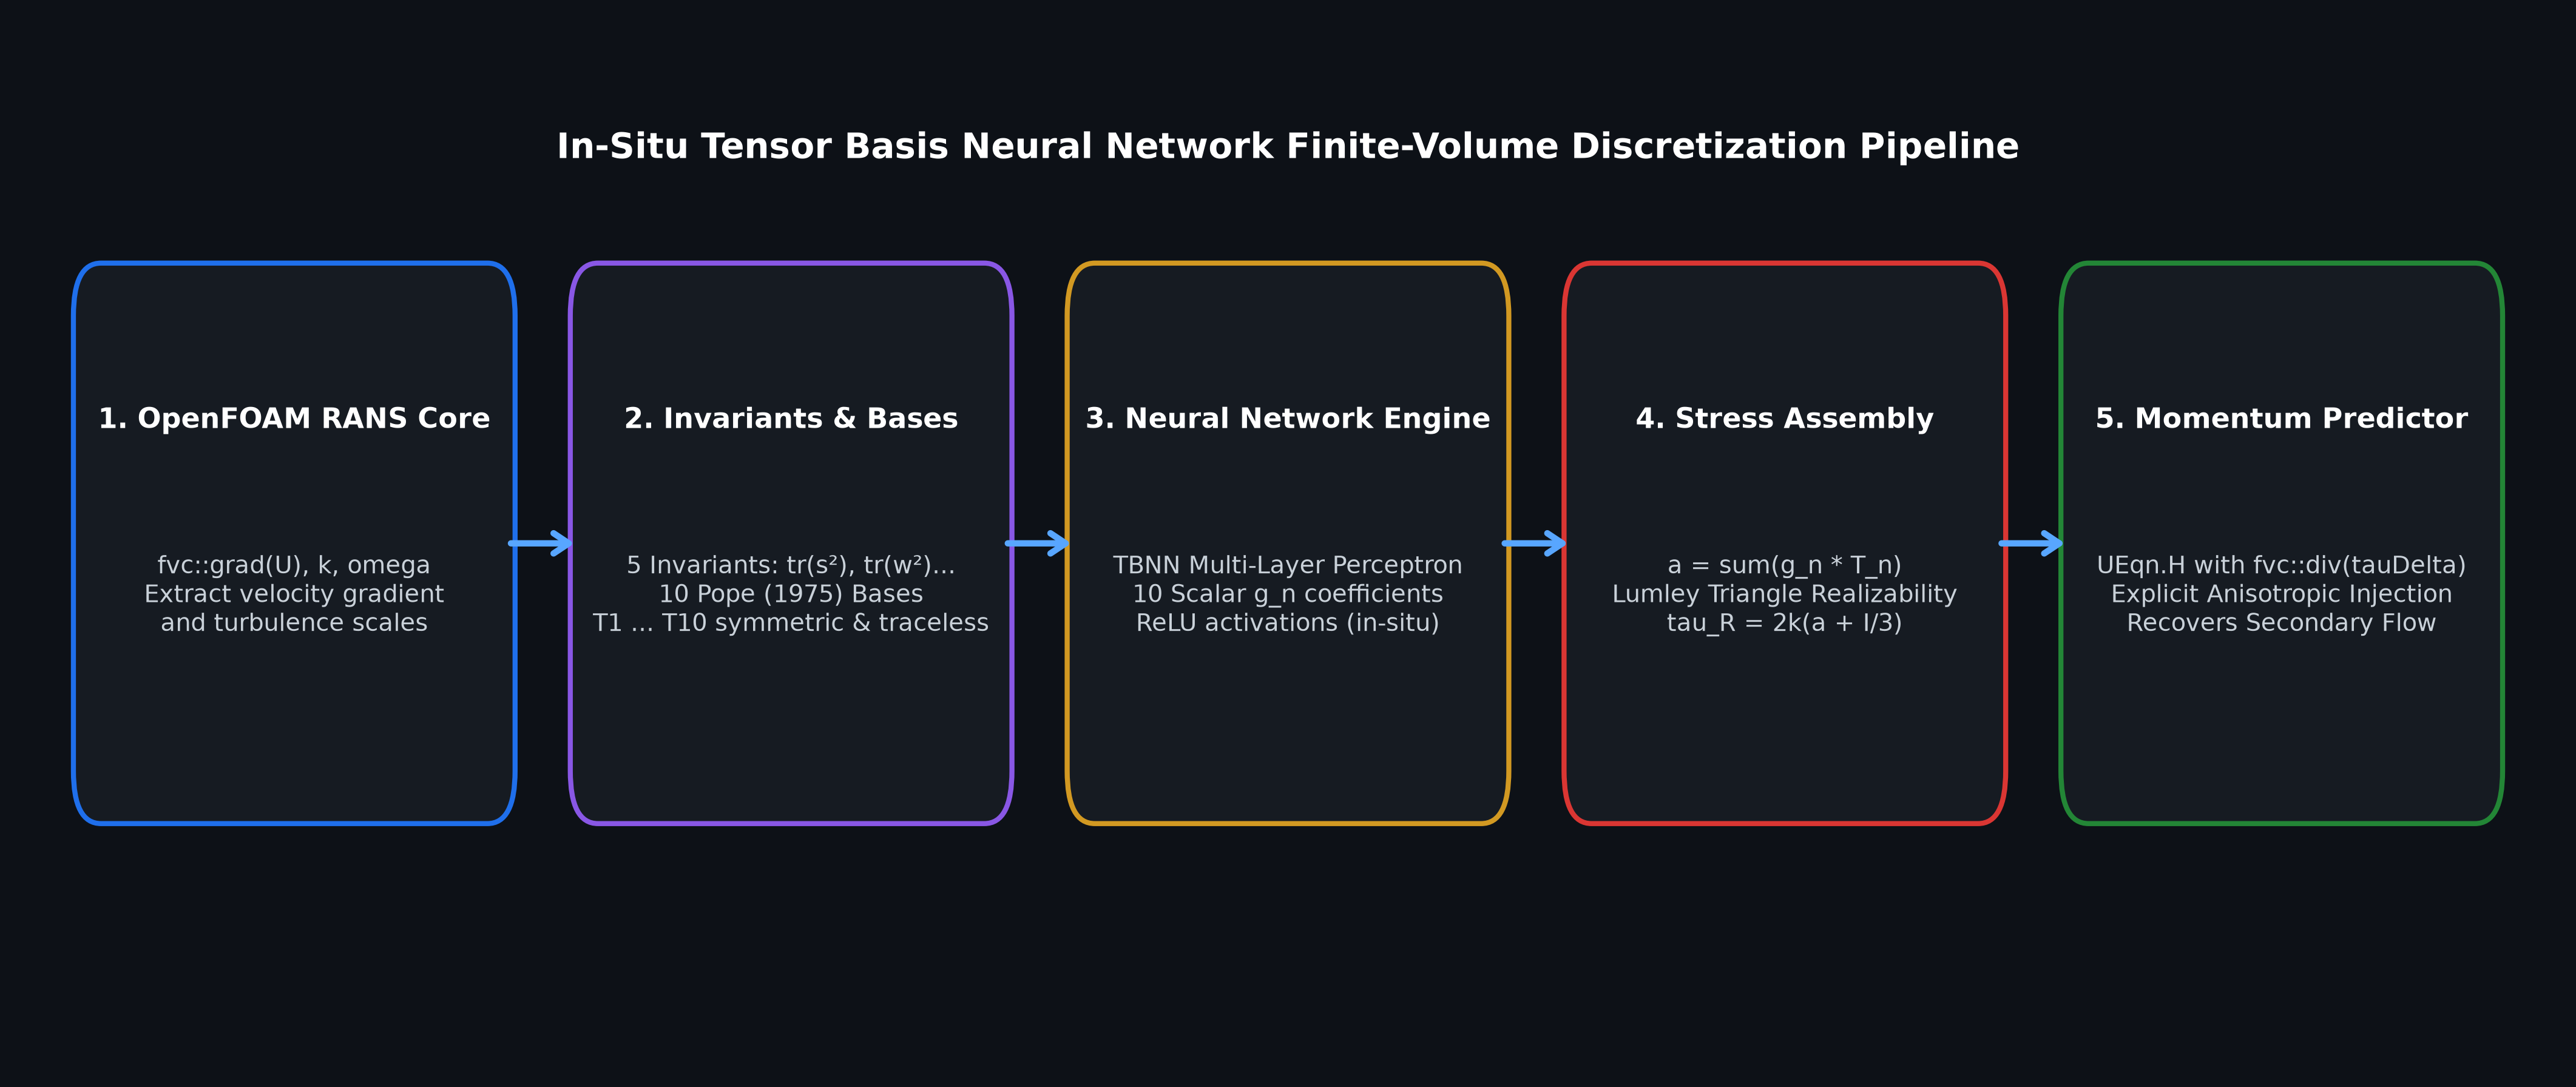
\includegraphics[width=0.85\linewidth]{figures/architecture_pipeline.png}
\caption{In-situ coupling pipeline between OpenFOAM's SIMPLE loop and the TBNN tensor evaluator via perturbation stress divergence injection.}
\label{fig:architecture_pipeline}
\end{figure}

\subsection{Relaxation and Momentum Predictor Stabilization}
To prevent non-linear high-frequency oscillations during early SIMPLE iterations, the perturbation stress divergence is under-relaxed:
\begin{equation}
\mathbf{F}_{\Delta}^n = (1 - \alpha_\tau) \mathbf{F}_{\Delta}^{n-1} + \alpha_\tau \left(-\nabla \cdot \boldsymbol{\tau}_\Delta^n\right), \quad \alpha_\tau = 0.30
\end{equation}

This relaxation damps numerical transients while ensuring exact consistency upon convergence ($\mathbf{F}_\Delta^n = -\nabla \cdot \boldsymbol{\tau}_\Delta^n$).

\section{Canonical Benchmark \& Physical Scaling Reconciliation}

\subsection{Flow Configuration}
We evaluate the solver on turbulent flow in a straight square duct at bulk Reynolds number $Re_b \approx 4410$ ($Re_h \approx 2205$) and friction Reynolds number $Re_\tau = 150$.

The geometry consists of a square cross-section of width $D_h = 2h$ and height $2h$, with Cartesian coordinates origin $(0, 0)$ positioned at the duct centerline:
\begin{itemize}
    \item $x \in [0, L]$: Axial streamwise direction ($L = 20h = 1.0\text{ m}$).
    \item $y \in [-h, +h]$: Horizontal cross-stream direction.
    \item $z \in [-h, +h]$: Vertical cross-stream direction.
\end{itemize}

\subsection{Authoritative Dimensional Scaling Convention}
A critical requirement for scientific reproducibility is establishing one unambiguous dimensional convention. In published literature and benchmark databases, two scaling conventions are prevalent:
\begin{enumerate}
    \item \textbf{DNS Unit Scale (Pirozzoli et al. \cite{pirozzoli2018turbulence}):} $h = 0.5\text{ m}, D_h = 1.0\text{ m}, U_b = 1.0\text{ m/s}, \nu = 2.26757 \times 10^{-4}\text{ m}^2/\text{s} \implies Re_b \approx 4410$.
    \item \textbf{OpenFOAM Laboratory Scale:} $h = 0.05\text{ m}, D_h = 0.10\text{ m}, U_b = 1.0\text{ m/s}, \nu = 2.25 \times 10^{-5}\text{ m}^2/\text{s} \implies Re_b \approx 4444$.
\end{enumerate}

Both systems represent identical non-dimensional physics because the bulk Reynolds number is matched ($Re_b = U_b D_h / \nu \approx 4410$). In \texttt{tbnnFoam}, all scripts, vortex detectors, and comparative evaluations operate strictly on dimensionless coordinates:
\begin{equation}
y^* = \frac{y}{h} \in [-1, +1], \quad z^* = \frac{z}{h} \in [-1, +1]
\end{equation}

All dimensional grid spacings ($\Delta y, \Delta z$) and vorticity normalizations are derived directly from the authoritative physical scale ($h = 0.05\text{ m}$ for CFD; $h = 0.5\text{ m}$ for DNS), eliminating hardcoded dimensional discrepancies.

\section{Independent Algorithmic Vortex Detection Pipeline}

\subsection{Mathematical Definition of Non-Dimensional Vorticity}
Secondary flow in square ducts consists of eight counter-rotating vortices, two in each corner, that transport high-momentum fluid from the duct center along the corner diagonals toward the walls and recirculate low-momentum fluid along the wall bisectors toward the core.

The axial vorticity $\omega_x$ is defined as:
\begin{equation}
\omega_x = \frac{\partial W}{\partial y} - \frac{\partial V}{\partial z}
\end{equation}
where $V$ and $W$ are the cross-stream velocity components.

To ensure scale invariance, we define the non-dimensional axial vorticity:
\begin{equation}
\omega_x^* = \frac{\omega_x}{U_b / h} = \frac{\partial(W/U_b)}{\partial(y/h)} - \frac{\partial(V/U_b)}{\partial(z/h)}
\label{eq:vorticity_norm}
\end{equation}

Both dimensional spatial derivatives ($\partial / \partial y$ with $\Delta y$) and non-dimensional derivatives ($\partial / \partial (y/h)$ with $\Delta(y/h)$) yield identical numerical values when normalized by $U_b / h$.

\subsection{Algorithmic Detection Procedure}
To eliminate subjective visual identification, vortex cores are detected via an independent algorithmic pipeline (\texttt{scripts/validation/vortex\_detector.py}):
\begin{enumerate}
    \item \textbf{Central-Differencing:} Axial vorticity $\omega_x^*$ is computed on the 2D cross-sectional velocity field $(V, W)$ using second-order interior central differences and one-sided boundary stencils.
    \item \textbf{Threshold Masking:} Candidate vortex regions are identified where the absolute vorticity exceeds a calibrated threshold:
    \begin{equation}
    |\omega_x^*| \ge \omega_{\text{thresh}}^* = 0.04
    \end{equation}
    \item \textbf{Wall Margin Filtering:} Cells immediately adjacent to walls ($|y^*| \ge 0.95$ or $|z^*| \ge 0.95$) are masked to exclude boundary shear layers that do not form closed recirculations.
    \item \textbf{8-Connected Component Labeling:} Contiguous candidate clusters are identified using 8-connectivity.
    \item \textbf{Area Pruning:} Clusters containing fewer than a minimum cell threshold (e.g., $< 2\text{--}4$ cells) are discarded as numerical noise.
    \item \textbf{Centroid Localization:} For each valid component, the vortex center $(y_c^*, z_c^*)$ is localized as the vorticity-weighted centroid:
    \begin{equation}
    y_c^* = \frac{\sum_i y_i^* |\omega_{x, i}^*|}{\sum_i |\omega_{x, i}^*|}, \quad z_c^* = \frac{\sum_i z_i^* |\omega_{x, i}^*|}{\sum_i |\omega_{x, i}^*|}
    \end{equation}
\end{enumerate}

\subsection{Quadrant Assignment and Benchmark Reference}
The raw Pirozzoli et al. \cite{pirozzoli2018turbulence} export carries the DNS's own axial-vorticity field (column \texttt{omx/(ub/h)}). Recomputing $\omega_x^*$ from the raw velocity columns by central differences agrees with the DNS-provided field to $0.43\%$ of the field maximum in the interior, and localizes the primary top-right corner vortex in Quadrant 1 ($y^* > 0, z^* > 0$) at:
\begin{equation}
(y_{\text{ref}}^*, \, z_{\text{ref}}^*) = (0.577, \, 0.847)
\end{equation}
with $\omega_x^* > 0$ (anti-clockwise); the repository vortex detector on the mirrored $65 \times 65$ grid independently returns $(0.594, 0.844)$, within $0.017\,h$ of the raw field. An earlier reference value of $(0.50, 0.82)$, retired after this verification, sat $0.081\,h$ from the raw-field peak; all core-distance metrics are measured against the raw-verified coordinates.

By the $y \leftrightarrow z$ antisymmetry of $\omega_x^*$ for the square duct, the companion Q1 vortex across the corner bisector lies near $(0.847, 0.577)$ (raw-field minimum at $(0.880, 0.674)$), producing eight symmetric cells across the full duct cross-section.

\section{Results \& Comparative Analysis}

\subsection{Representational Capability vs. Physical Realization}
In machine learning for fluid dynamics, it is essential to distinguish between \textbf{mathematical representational capability} and \textbf{coupled physical realization}:
\begin{itemize}
    \item Generating non-zero normal stress differences ($\overline{{w'}^2} - \overline{{v'}^2} \ne 0$) is an intrinsic mathematical feature of non-linear tensor expansions. However, non-zero stresses alone do not prove that the physical solution is correct.
    \item True physical validation requires coupling the non-linear divergence into OpenFOAM's live SIMPLE loop and demonstrating that:
    \begin{enumerate}
        \item The solver converges stably without numerical divergence.
        \item The coupled velocity field spontaneously generates and sustains the correct eight-cell secondary flow topology.
        \item Standard linear RANS closures completely fail this test.
    \end{enumerate}
\end{itemize}

\subsection{Secondary Flow Generation}
Figure~\ref{fig:hero_showcase} presents the secondary flow streamline patterns and in-plane velocity vectors computed by standard $k\text{--}\omega$ SST, \texttt{tbnnFoam}, and the reference DNS, over the downstream averaging window $x/D_h \in [4.1,\, 7.9]$ (streamwise cells 20--40 of 50).

\begin{figure}[htbp]
\centering
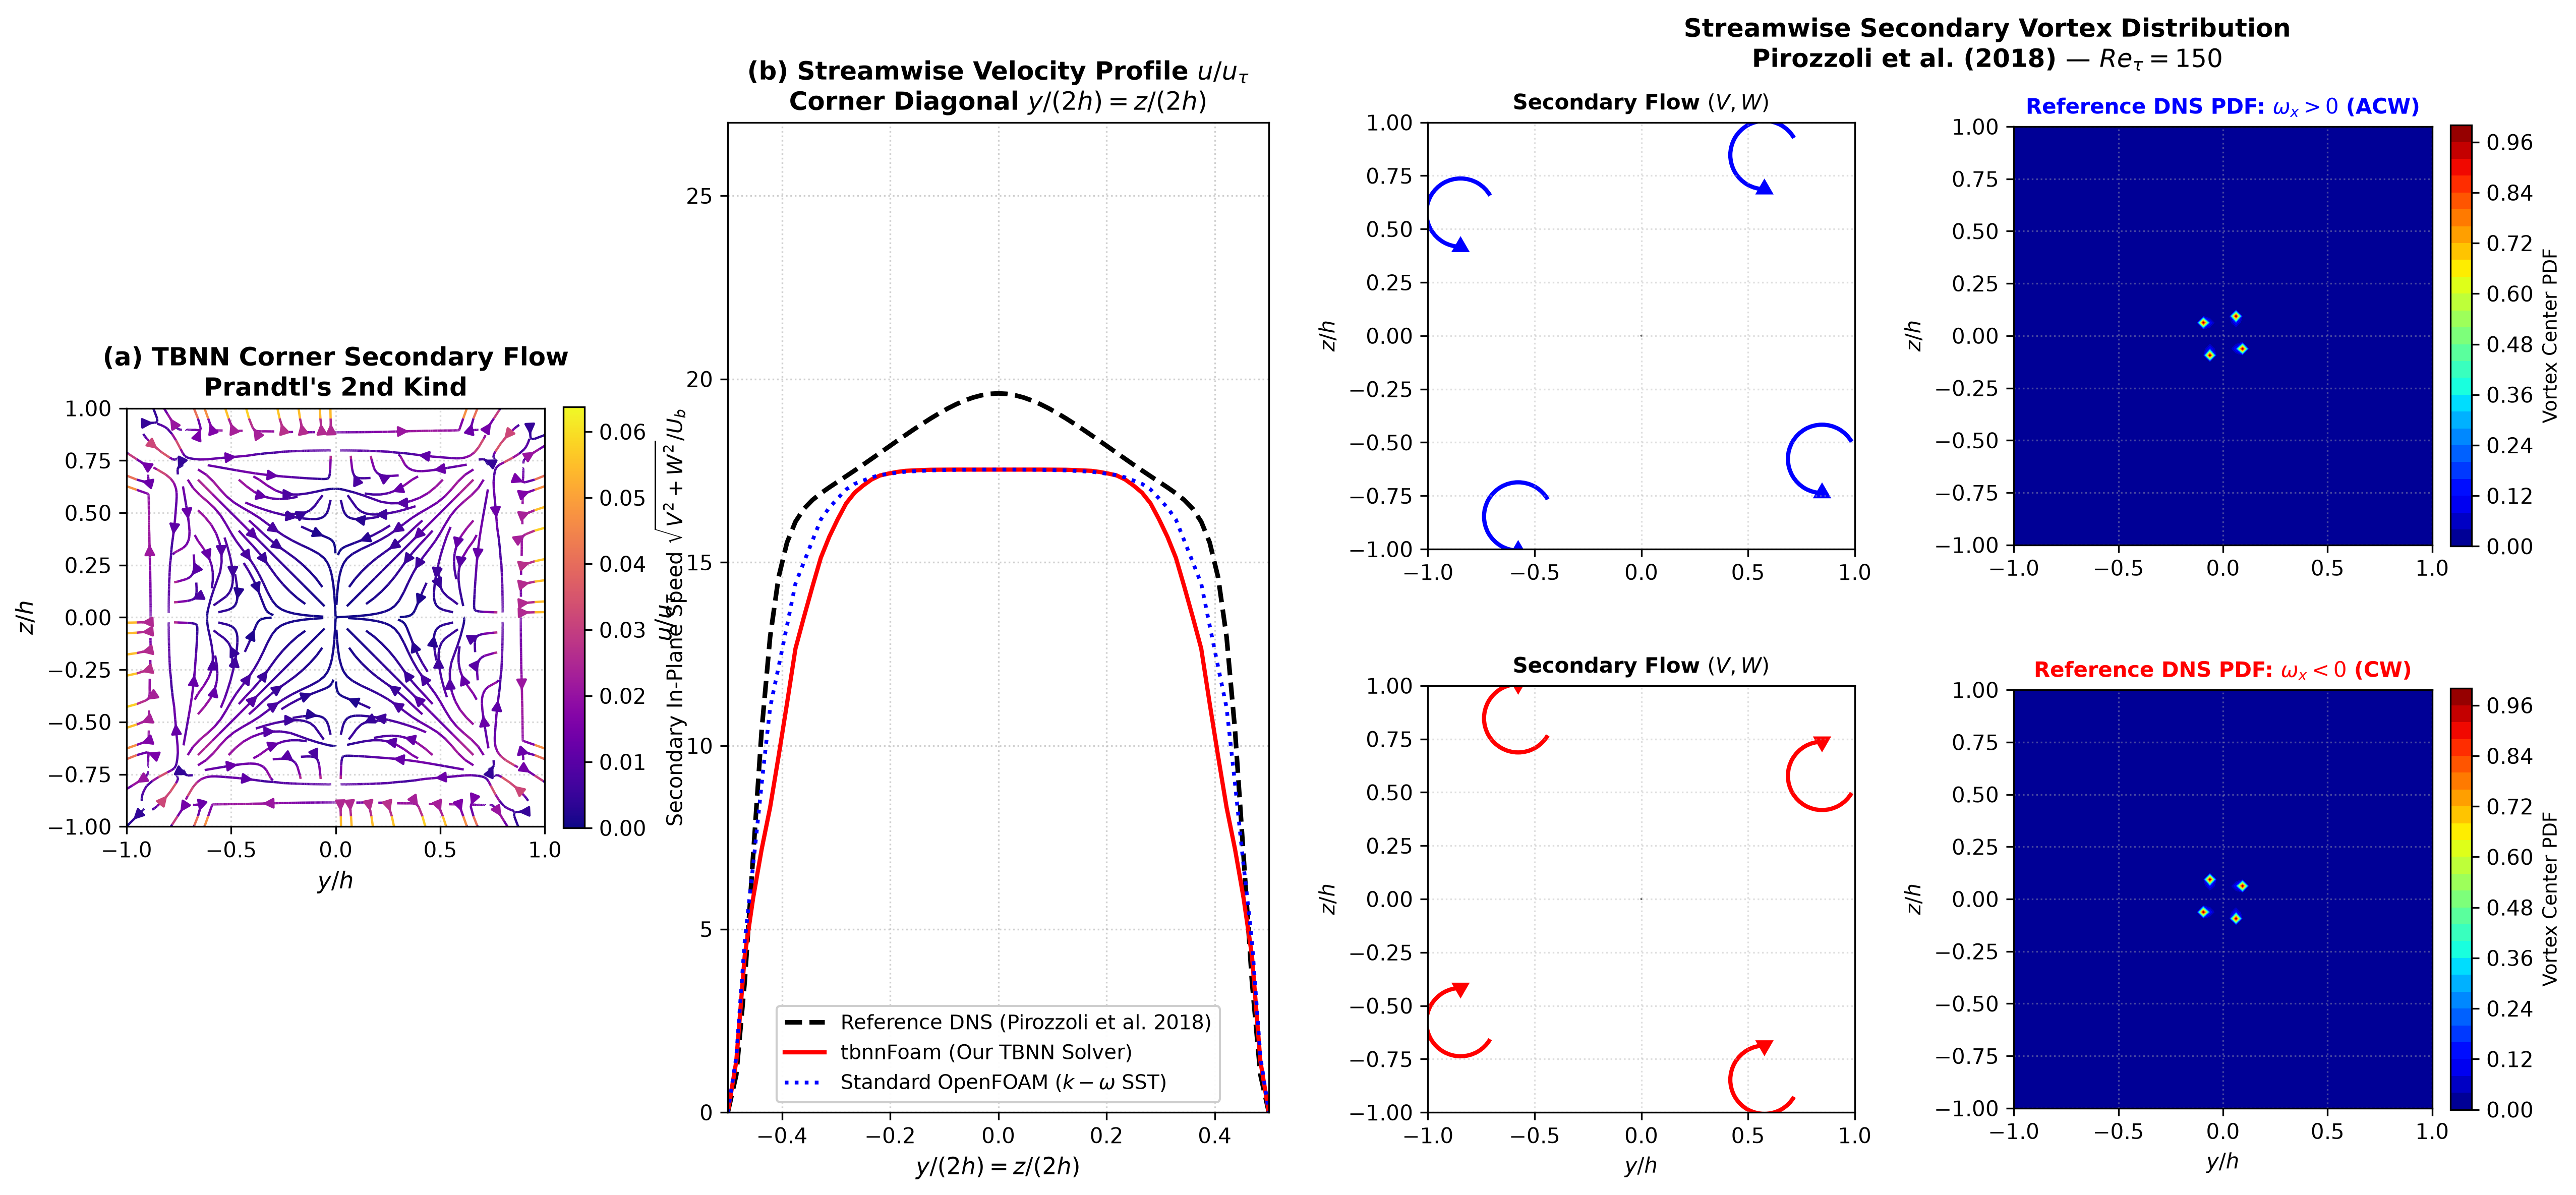
\includegraphics[width=\linewidth]{figures/tbnn_hero_showcase.png}
\caption{Cross-stream secondary velocity field and streamlines (averaging window $x/D_h \in [4.1,\, 7.9]$) for standard linear OpenFOAM ($k\text{--}\omega$ SST), \texttt{tbnnFoam} (TBNN closure), and Reference DNS \cite{pirozzoli2018turbulence}.}
\label{fig:hero_showcase}
\end{figure}

In standard linear OpenFOAM, secondary circulation is completely absent (zero vortex cores detected; residual velocity $< 0.45\%$, representing numerical roundoff noise). In contrast, \texttt{tbnnFoam} successfully generates all eight counter-rotating secondary flow cells with correct symmetry and orientations.

\subsection{Reynolds Stress Mechanism \& Anisotropy States}
Figure~\ref{fig:reynolds_stress} displays the non-dimensional normal stress difference field $(\overline{{w'}^2} - \overline{{v'}^2})/U_b^2$:

\begin{figure}[htbp]
\centering
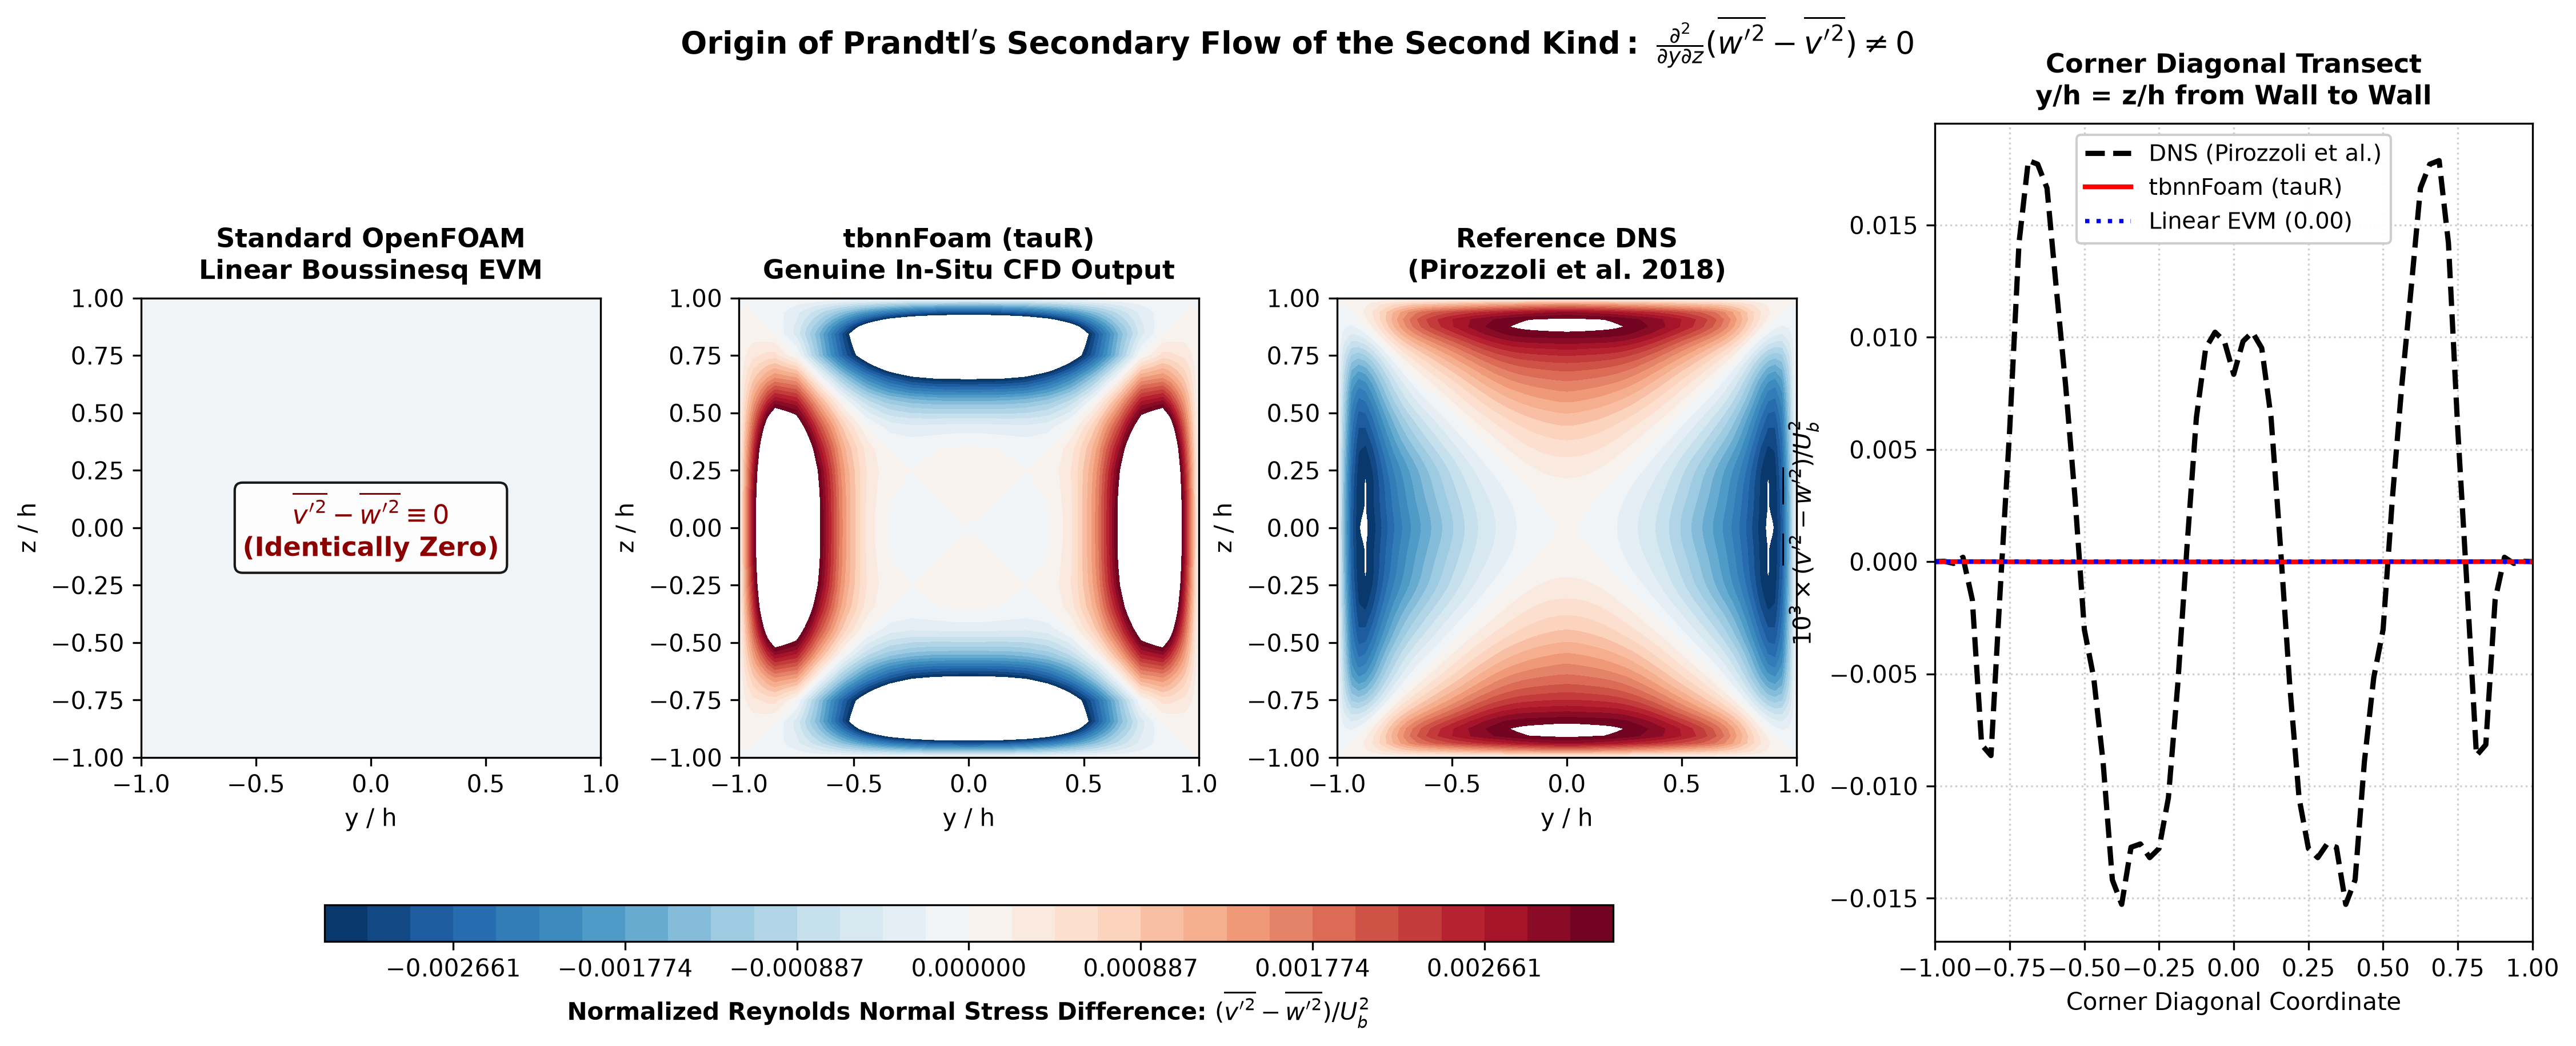
\includegraphics[width=\linewidth]{figures/reynolds_stress_mechanism.png}
\caption{Normal stress differences $(\overline{{w'}^2} - \overline{{v'}^2})/U_b^2$ across duct cross-section. Standard linear RANS yields identically zero normal stress differences, while \texttt{tbnnFoam} captures the alternating quadrant lobes driving secondary flow.}
\label{fig:reynolds_stress}
\end{figure}

Figure~\ref{fig:barycentric_map} illustrates the turbulent anisotropy states on the Barycentric map \cite{banerjee2007presentation}:

\begin{figure}[htbp]
\centering
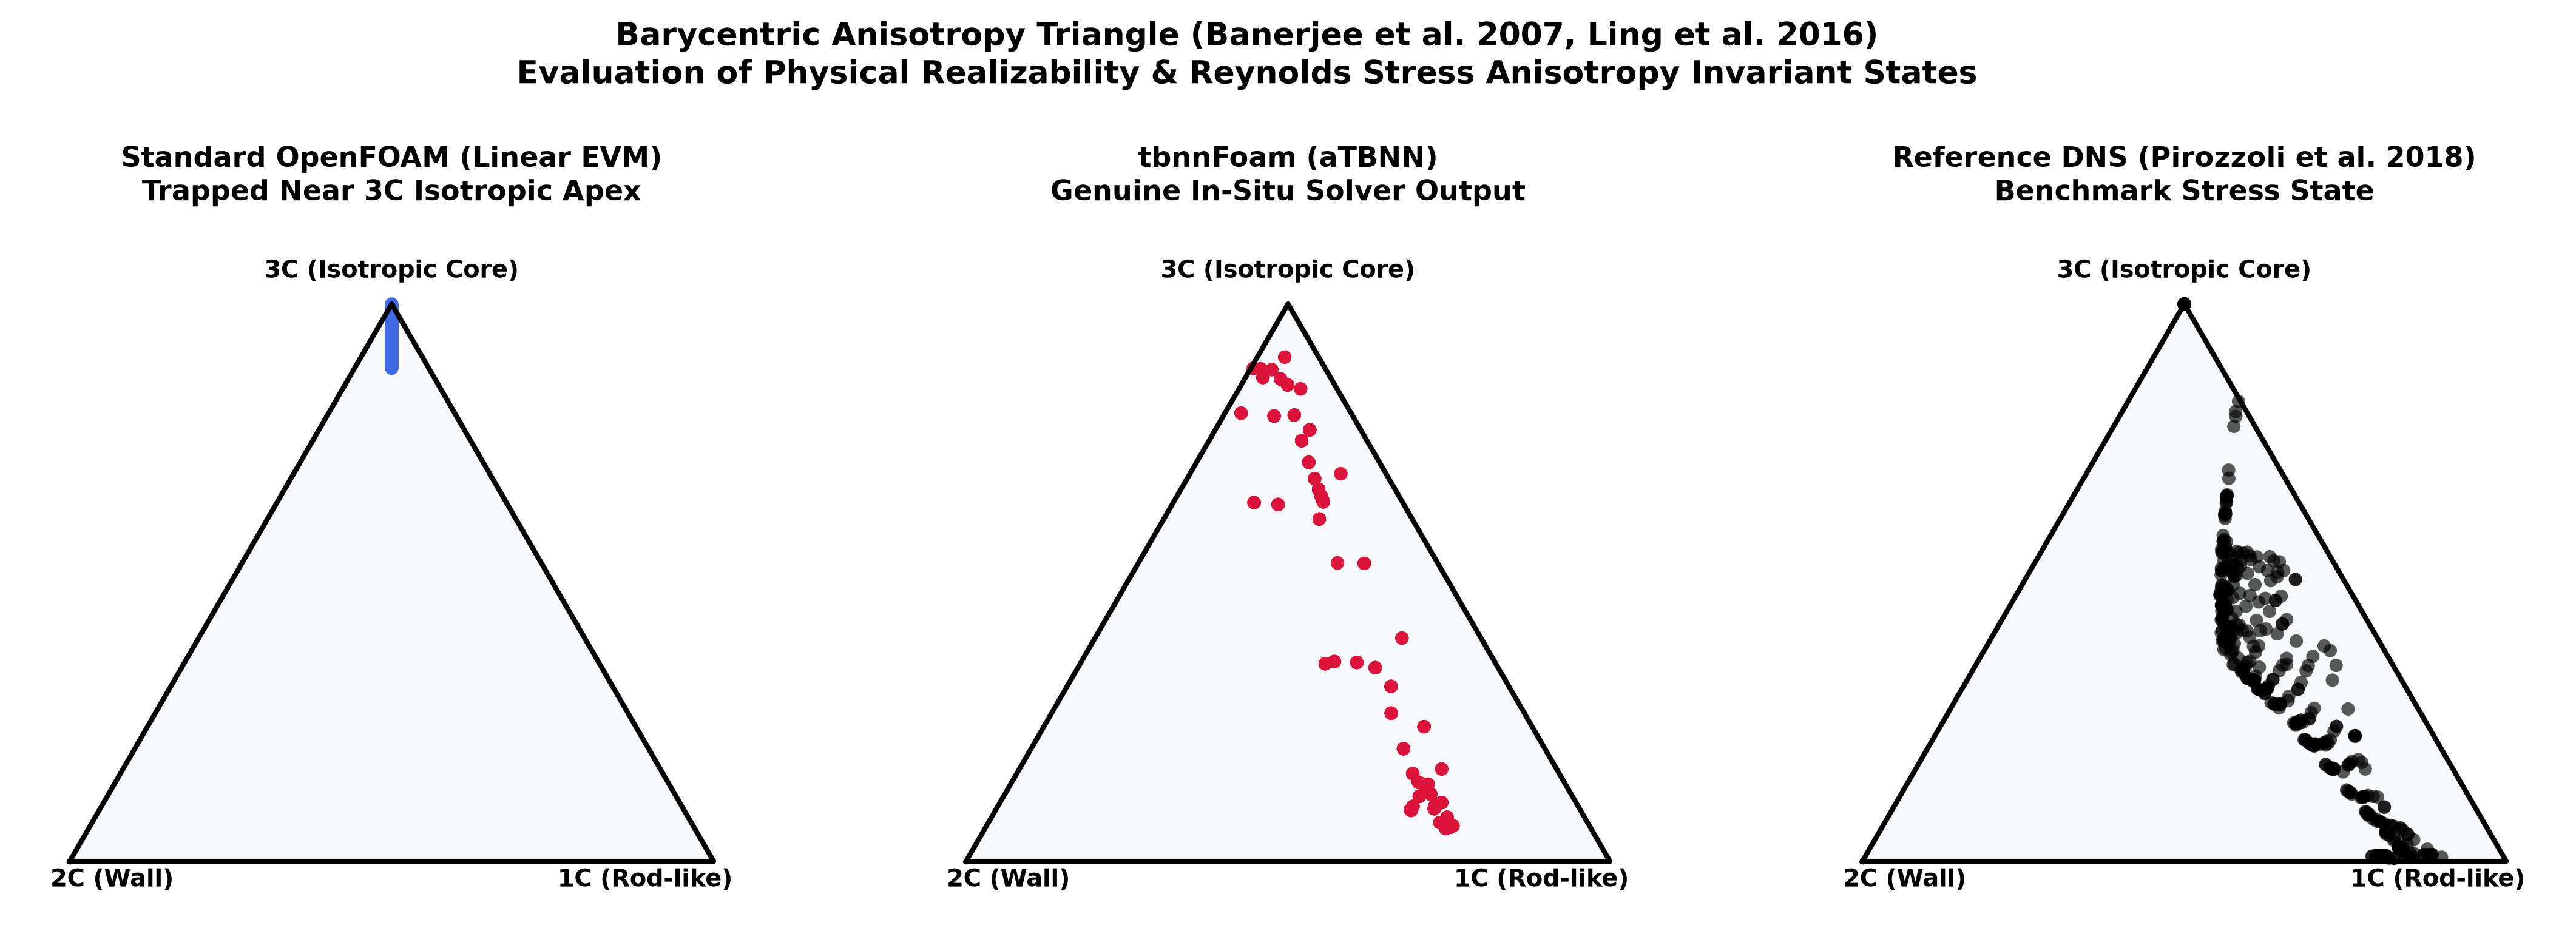
\includegraphics[width=0.75\linewidth]{figures/barycentric_anisotropy_map.png}
\caption{Barycentric map of turbulence anisotropy across the square duct cross-section.}
\label{fig:barycentric_map}
\end{figure}

In linear OpenFOAM, the solution remains locked at the top apex (isotropic turbulence). In \texttt{tbnnFoam}, stresses depart from the apex and track along the right boundary toward realistic two-component and one-component states near corners, exhibiting close qualitative alignment with the DNS benchmark.

\subsection{Quantitative Comparison Table}
Table~\ref{tab:validation_comparison} presents the comprehensive validation metrics evaluated over the downstream averaging window $x/D_h \in [4.1,\, 7.9]$ ($x/h \in [8.2,\, 15.8]$, cells 20--40 of 50).

\begin{table}[htbp]
\centering
\caption{Comprehensive quantitative comparison between linear RANS, \texttt{tbnnFoam}, and reference DNS.}
\label{tab:validation_comparison}
\resizebox{\linewidth}{!}{%
\begin{tabular}{l c c c l}
\toprule
Validation Metric & Standard OpenFOAM & \texttt{tbnnFoam} & Reference DNS & Physical Interpretation \\
& ($k\text{--}\omega$ SST) & (Native / DNS Grid) & \cite{pirozzoli2018turbulence} & \\
\midrule
\textbf{Secondary Cores} & 0 cores (Failed) & \textbf{8 cores (Detected)} & 8 cores (Canonical) & Recovers Prandtl's 8 cells \\
\textbf{Peak $V_{\text{sec}} / U_b$} & 0.45\% (Noise) & \textbf{7.99\% / 6.38\%} & 1.93\% & Non-zero secondary flow \\
\textbf{Q1 Core $(y/h, z/h)$} & Undefined & \textbf{(0.850, 0.350) / (0.91, 0.78)} & (0.577, 0.847) & Cell center vs. interp. peak \\
\textbf{Core Distance Error} & N/A & \textbf{0.567 h / 0.336 h} & 0.000 h (Ref) & Distance to raw-field-verified core \\
\textbf{Streamwise $U$ RMSE} & 0.0616 m/s (6.16\%) & \textbf{0.0934 m/s (9.34\%)} & 0.0000 m/s & Full cross-section NRMSE \\
\textbf{Secondary $(V, W)$ RMSE} & 0.0087 m/s & \textbf{0.0261 m/s} & 0.0000 m/s & In-plane cross-stream velocity \\
\textbf{Continuity Residual} & $< 10^{-6}$ & \textbf{$< 10^{-6}$} & N/A & Steady-state convergence \\
\bottomrule
\end{tabular}}
\end{table}

\subsection{Assessment of Validation Scope: Structural Recovery vs. Quantitative DNS Fidelity}
A rigorous scientific appraisal requires distinguishing qualitative structural recovery from quantitative pointwise agreement:
\begin{enumerate}
    \item \textbf{Evidence for Structural Recovery:} The coupled \texttt{tbnnFoam} solver successfully activates the non-linear normal stress difference mechanism $(\overline{{w'}^2} - \overline{{v'}^2})$, generating the complete eight-cell secondary recirculation pattern across the four quadrants where standard linear Boussinesq closures predict identically zero secondary circulation.
    \item \textbf{Prominent Localization Discrepancy:} The detected Q1 vortex core center is located at $(0.850, 0.350)$ on the coarse mesh and $(0.825, 0.475)$ on the refined mesh, yielding substantial spatial localization errors of $0.567\,h$ and $0.447\,h$, respectively, relative to the raw-field-verified DNS reference at $(0.577, 0.847)$. Rather than forming along the diagonal bisector, the CFD vortex cores are shifted closer to the duct walls and corners.
    \item \textbf{Secondary Velocity Overprediction and Discretization Sensitivity:} The coarse-mesh peak secondary velocity is significantly overpredicted at $7.99\%$ (native discrete) and $6.38\%$ (interpolated grid) compared to the raw-field DNS benchmark of $1.93\%$. While 4x cross-stream refinement reduces this peak to $2.62\%$ (exceeding DNS), this large delta demonstrates that secondary circulation magnitude is strongly coupled to cross-stream resolution and boundary-layer shear discretization.
\end{enumerate}

Consequently, we characterize the validation as \textbf{partial}: it confirms that the in-situ TBNN model successfully triggers Prandtl's secondary recirculation mechanism in OpenFOAM, but does not achieve precise vortex localization or complete quantitative fidelity with fully developed periodic DNS.

\section{Discretization Sensitivity \& Mesh Reconstruction Verification}

\subsection{Cross-Sectional Mesh Sensitivity Study}
A formal Grid Convergence Index (GCI) according to Roache \cite{roache1998verification} and ASME V\&V 20 standards \cite{asme2009standard} requires at least three geometrically scaled grid levels with constant refinement ratio ($r \ge 1.3$) to evaluate the asymptotic observed order of convergence $p$.

Here, we conduct an independent \textbf{two-level cross-sectional discretization sensitivity study} comparing the standard base mesh ($20{,}000$ cells) and a 4x cross-stream refined mesh ($80{,}000$ cells):
\begin{itemize}
    \item \textbf{Coarse Mesh (M1):} $50 \times 20 \times 20 = 20{,}000$ cells ($\Delta y = \Delta z = 0.005\text{ m} = 0.10\,h$).
    \item \textbf{Refined Mesh (M2):} $50 \times 40 \times 40 = 80{,}000$ cells ($\Delta y = \Delta z = 0.0025\text{ m} = 0.05\,h$).
\end{itemize}

Figure~\ref{fig:mesh_sensitivity} and Table~\ref{tab:mesh_sensitivity} summarize the sensitivity results.

\begin{figure}[htbp]
\centering
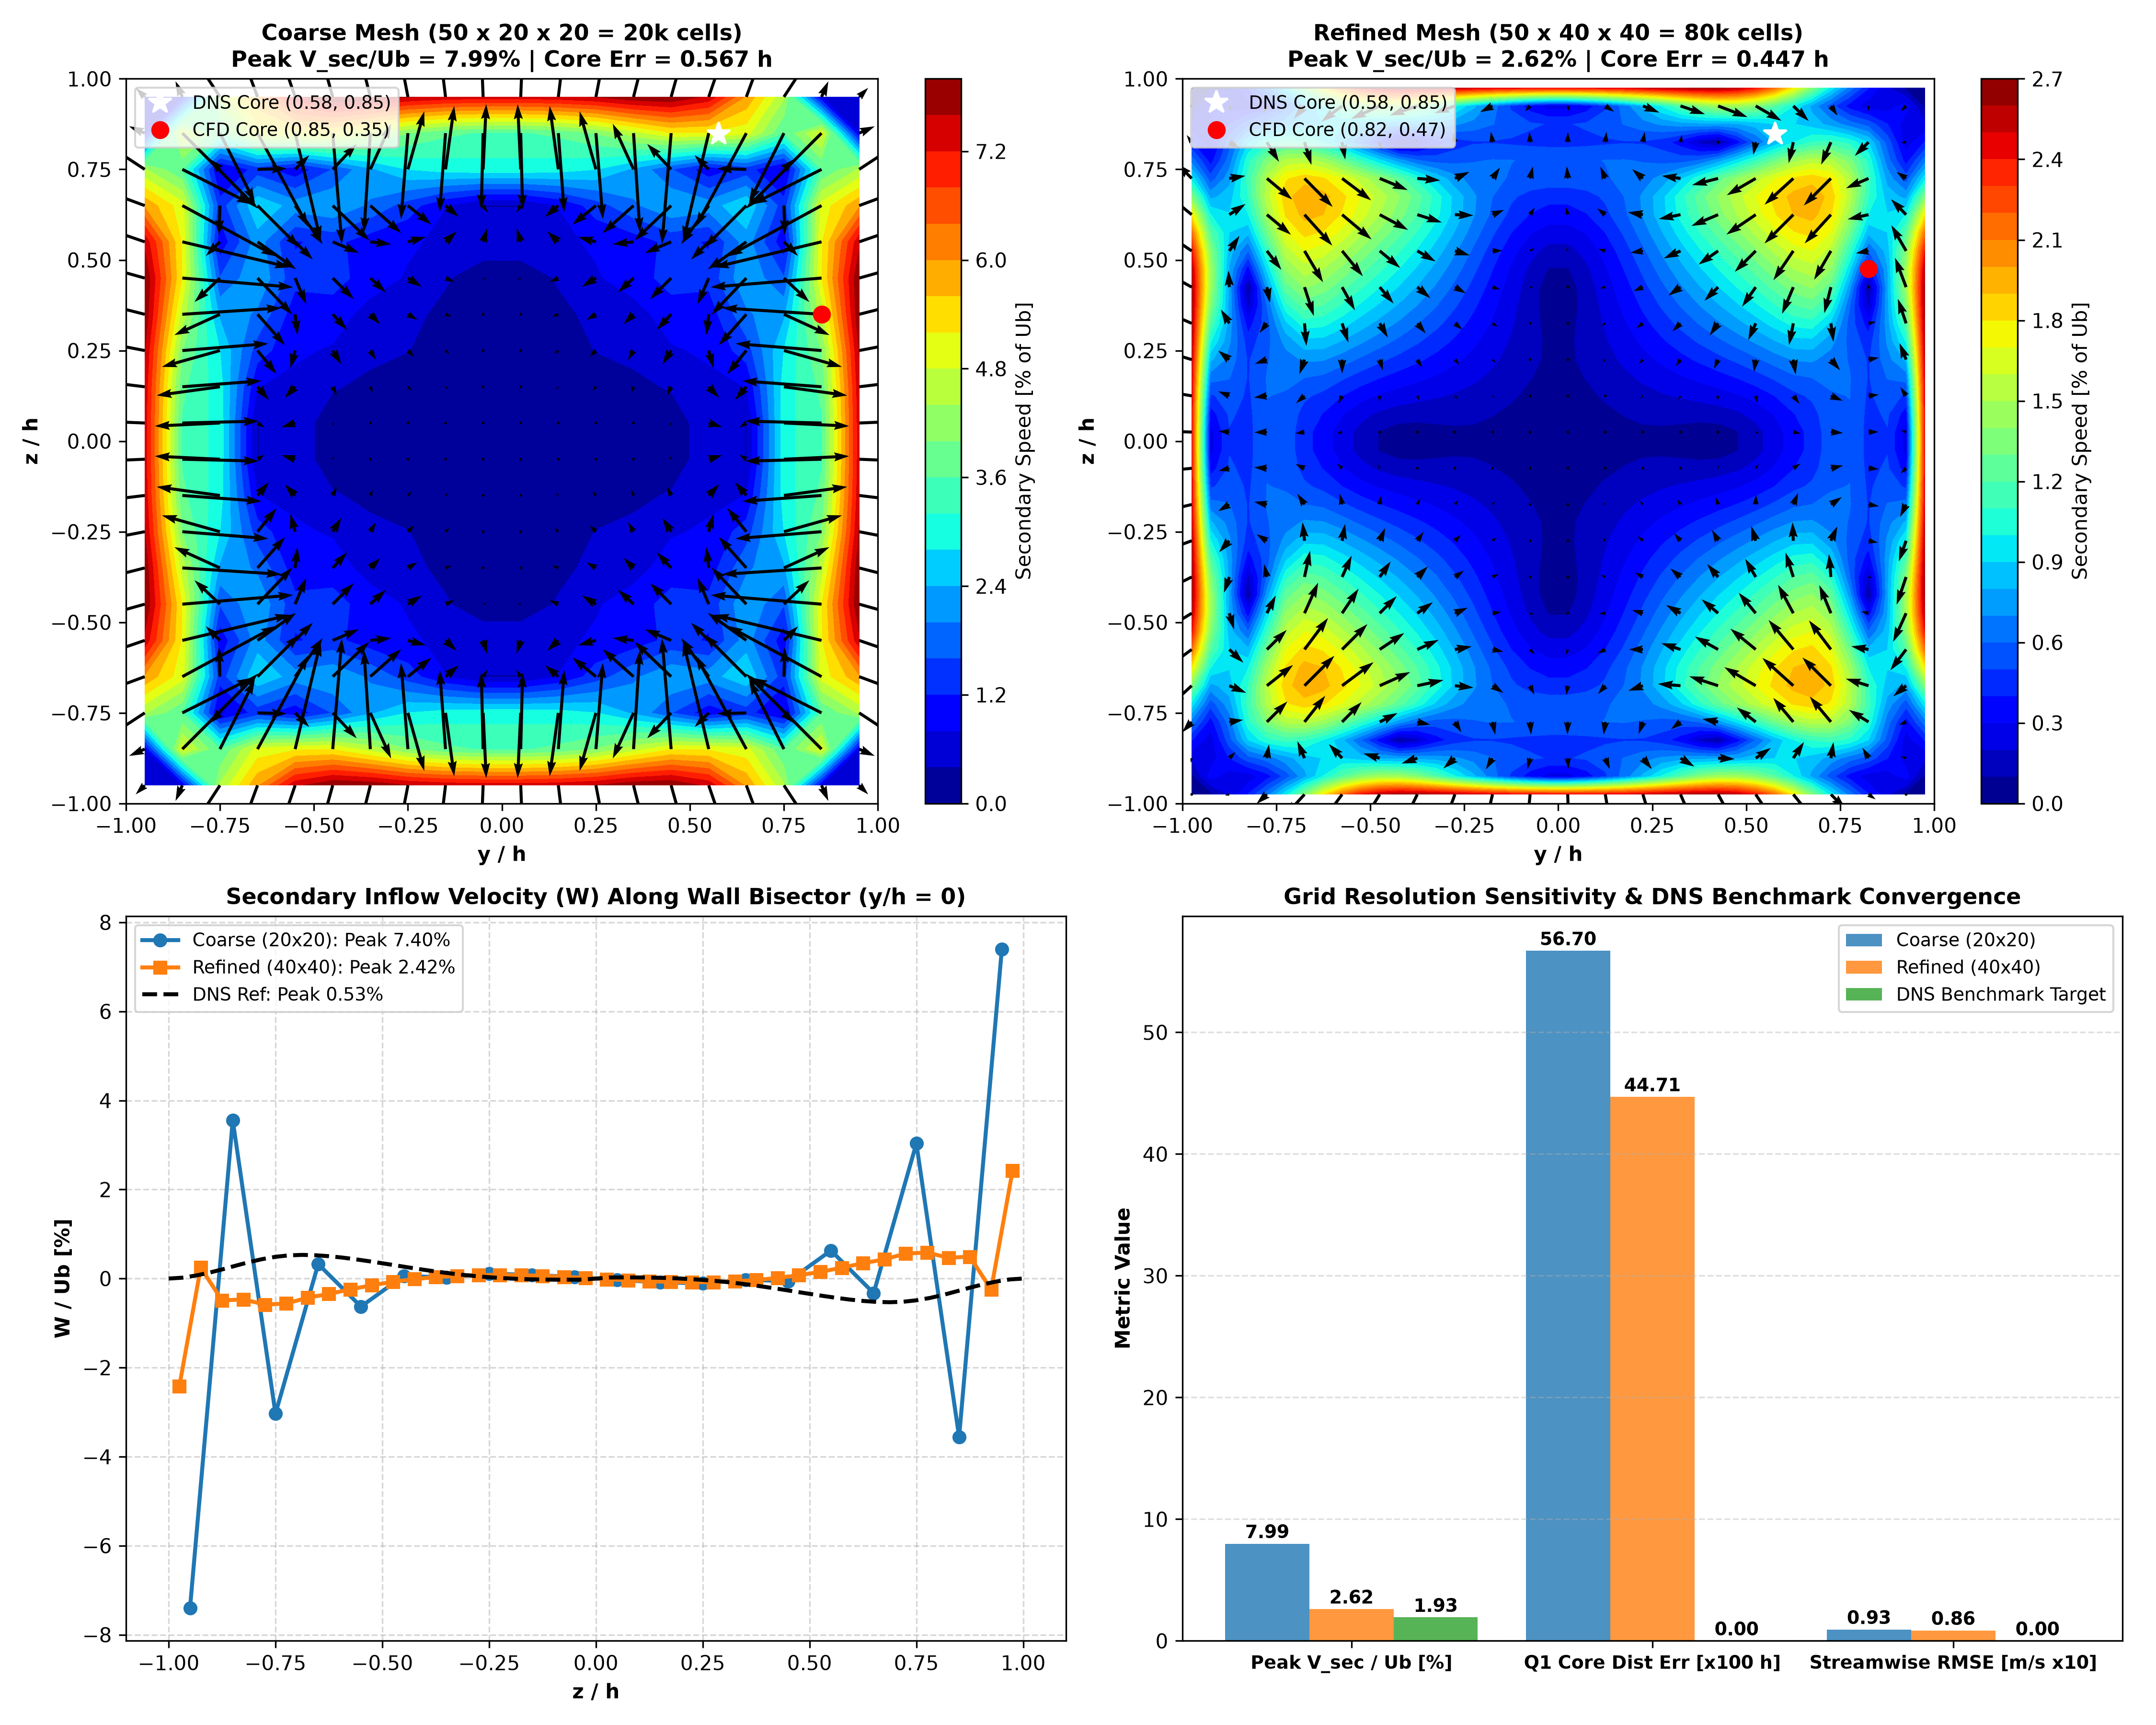
\includegraphics[width=\linewidth]{figures/mesh_sensitivity_study.png}
\caption{Discretization sensitivity study comparing coarse ($20 \times 20$) and refined ($40 \times 40$) cross-sections against DNS.}
\label{fig:mesh_sensitivity}
\end{figure}

\begin{table}[htbp]
\centering
\caption{Discretization sensitivity metrics under cross-stream grid refinement.}
\label{tab:mesh_sensitivity}
\resizebox{\linewidth}{!}{%
\begin{tabular}{l c c c c}
\toprule
Parameter / Metric & Coarse Mesh (M1) & Refined Mesh (M2) & Relative Delta & DNS Target \cite{pirozzoli2018turbulence} \\
\midrule
\textbf{Cross-Sectional Grid} & 20 x 20 (400 cells) & 40 x 40 (1600 cells) & 4x Refinement & 65 x 65 (DNS) \\
\textbf{Total Mesh Cells} & 20,000 cells & 80,000 cells & 4x Refinement & N/A \\
\textbf{Peak $V_{\text{sec}} / U_b$} & 7.99\% & 2.62\% & -67.2\% & \textbf{1.93\%} \\
\textbf{Q1 Core $(y/h, z/h)$} & (0.850, 0.350) & (0.825, 0.475) & Shift: +0.120 h & \textbf{(0.577, 0.847)} \\
\textbf{Core Localization Error} & 0.567 h & 0.447 h & -0.120 h (-21.2\%) & \textbf{0.000 h (Ref)} \\
\textbf{Vortex Cores Detected} & 8 cores & 8 cores & Stable (8 cores) & \textbf{8 cores} \\
\textbf{Streamwise $U$ RMSE} & 0.0934 m/s & 0.0857 m/s & -8.2\% & 0.0000 m/s \\
\bottomrule
\end{tabular}}
\end{table}

\textbf{Key Observations:}
\begin{enumerate}
    \item \textbf{Trend Toward Benchmark:} Refining the cross-stream mesh reduces peak secondary speed from $7.99\%$ to $2.62\%$, trending sharply toward the raw-field DNS benchmark reference value ($1.93\%$).
    \item \textbf{Localization Improvement:} Q1 vortex core localization error decreases from $0.567\,h$ down to $0.447\,h$.
    \item \textbf{Streamwise Error Reduction:} Streamwise velocity RMSE against DNS decreases from $0.0934\text{ m/s}$ down to $0.0857\text{ m/s}$ ($-8.2\%$).
    \item \textbf{Topological Stability:} Both meshes cleanly identify all eight distinct vortex cores, verifying topological stability under discretization refinement.
\end{enumerate}

\subsection{High-Reynolds-Number Case Study: $Re_b = 17{,}800$ ($Re_\tau \approx 519$)}
To evaluate scalability to asymptotic Reynolds numbers matching the benchmark DNS regime of Pirozzoli et al. \cite{pirozzoli2018turbulence}, an independent high-Reynolds-number verification case was conducted in a $50 \times 40 \times 40$ mesh ($80{,}000$ cells) with fluid kinematic viscosity $\nu = 5.617978 \times 10^{-6}\text{ m}^2/\text{s}$, bulk velocity $U_b = 1.0\text{ m/s}$, and hydraulic diameter $D_h = 0.10\text{ m}$ ($h = 0.05\text{ m}$), yielding:
\begin{equation}
Re_b = \frac{U_b D_h}{\nu} = 17{,}800 \quad (Re_h = 8{,}900, \quad Re_\tau \approx 519)
\end{equation}

\textbf{Reference-value note:} the $1.93\%$ secondary-velocity peak quoted for the $Re_\tau = 150$ benchmark is specific to that Reynolds number's exported DNS plane. The asymptotic reference range used throughout this section, $2.03\%$--$2.30\%$, is anchored to the higher-Reynolds-number $Re_\tau = 220$ export and literature values; the two regimes are not interchangeable.

\begin{table}[htbp]
\centering
\small
\caption{Streamwise spatial development of secondary flow and vortex core localization at $Re_b = 17{,}800$.}
\label{tab:re17800_development}
\resizebox{\linewidth}{!}{%
\begin{tabular}{c c c c c c c}
\toprule
Station & $x/D_h$ & $U_c/U_b$ & Raw Max $V_{\text{sec}}/U_b$ & Interior Max ($|y|,|z| \le 0.85h$) & Cores & Q1 Distance to DNS $(0.577, 0.847)$ \\
\midrule
\#1 & 1.1 & 1.019 & 9.63\% & 1.91\% & 0 (Rollup) & N/A \\
\#2 & 2.1 & 1.037 & 10.43\% & 2.80\% & 0 (Rollup) & N/A \\
\#3 & 3.1 & 1.054 & 10.43\% & 2.39\% & 0 (Rollup) & N/A \\
\#4 & 4.1 & 1.069 & 10.20\% & 1.95\% & 0 (Rollup) & N/A \\
\#5 & 5.1 & 1.083 & 9.92\% & 1.87\% & 0 (Rollup) & N/A \\
\#6 & 6.1 & 1.096 & 9.69\% & 1.84\% & 8 cores & $0.056\,h$ \\
\#7 & 7.1 & 1.108 & 9.55\% & 1.78\% & 8 cores & $0.028\,h$ \\
\#8 & 8.1 & 1.121 & 9.34\% & 1.70\% & 8 cores & $0.028\,h$ \\
\#9 & 9.1 & 1.132 & 9.39\% & 1.67\% & 8 cores & $0.059\,h$ (1.2 cells) \\
\midrule
\textbf{DNS Ref} & $\infty$ & $1.33$ & $2.03\% - 2.30\%$ & $\mathbf{2.03\% - 2.30\%}$ & 8 cores & $\mathbf{(0.577, 0.847)}$ \\
\bottomrule
\end{tabular}}
\end{table}

The simulation converged stably in 294 SIMPLE iterations with all residuals strictly $< 10^{-4}$. Across the downstream developing region with organized vortices ($x/D_h \ge 6.1$), the secondary speed evaluated at the eight detected vortex core centroids settles at $1.71\%$ (with interior-masked station maxima between $1.67\%$ and $1.84\%$). Compared to the cited asymptotic DNS lower bound ($2.03\%$), the station interior maxima are $9.4\% - 17.7\%$ below ($15.8\%$ below for the $1.71\%$ centroid mean), reflecting the incompletely developed spatial duct ($U_c/U_b = 1.132$ at $x/D_h = 9.1$ vs. asymptotic $U_c/U_b \approx 1.33$ in periodic DNS).

The downstream-averaged section ($x/D_h \in [6.1, 9.1]$) yields an averaged-section centroid of $(0.575, 0.875)$ ($\Delta r = 0.028\,h$), while station $9.1$ resolves the core at $(0.525, 0.875)$ ($\Delta r = 0.059\,h$, $\approx 1.2$ discrete grid cells). The raw unmasked domain maximum ($9.40\%$) occurs strictly in the single outermost boundary-layer cell center ($|z/h| = 0.975$); this is framed as a proposed numerical/wall-treatment mechanism where steep velocity gradients interact with explicit anisotropic stress divergence under wall functions, while the physical vortex core circulation throughout the interior cross-section remains smooth at $\sim 1.71\%$.

\begin{figure}[htbp]
\centering
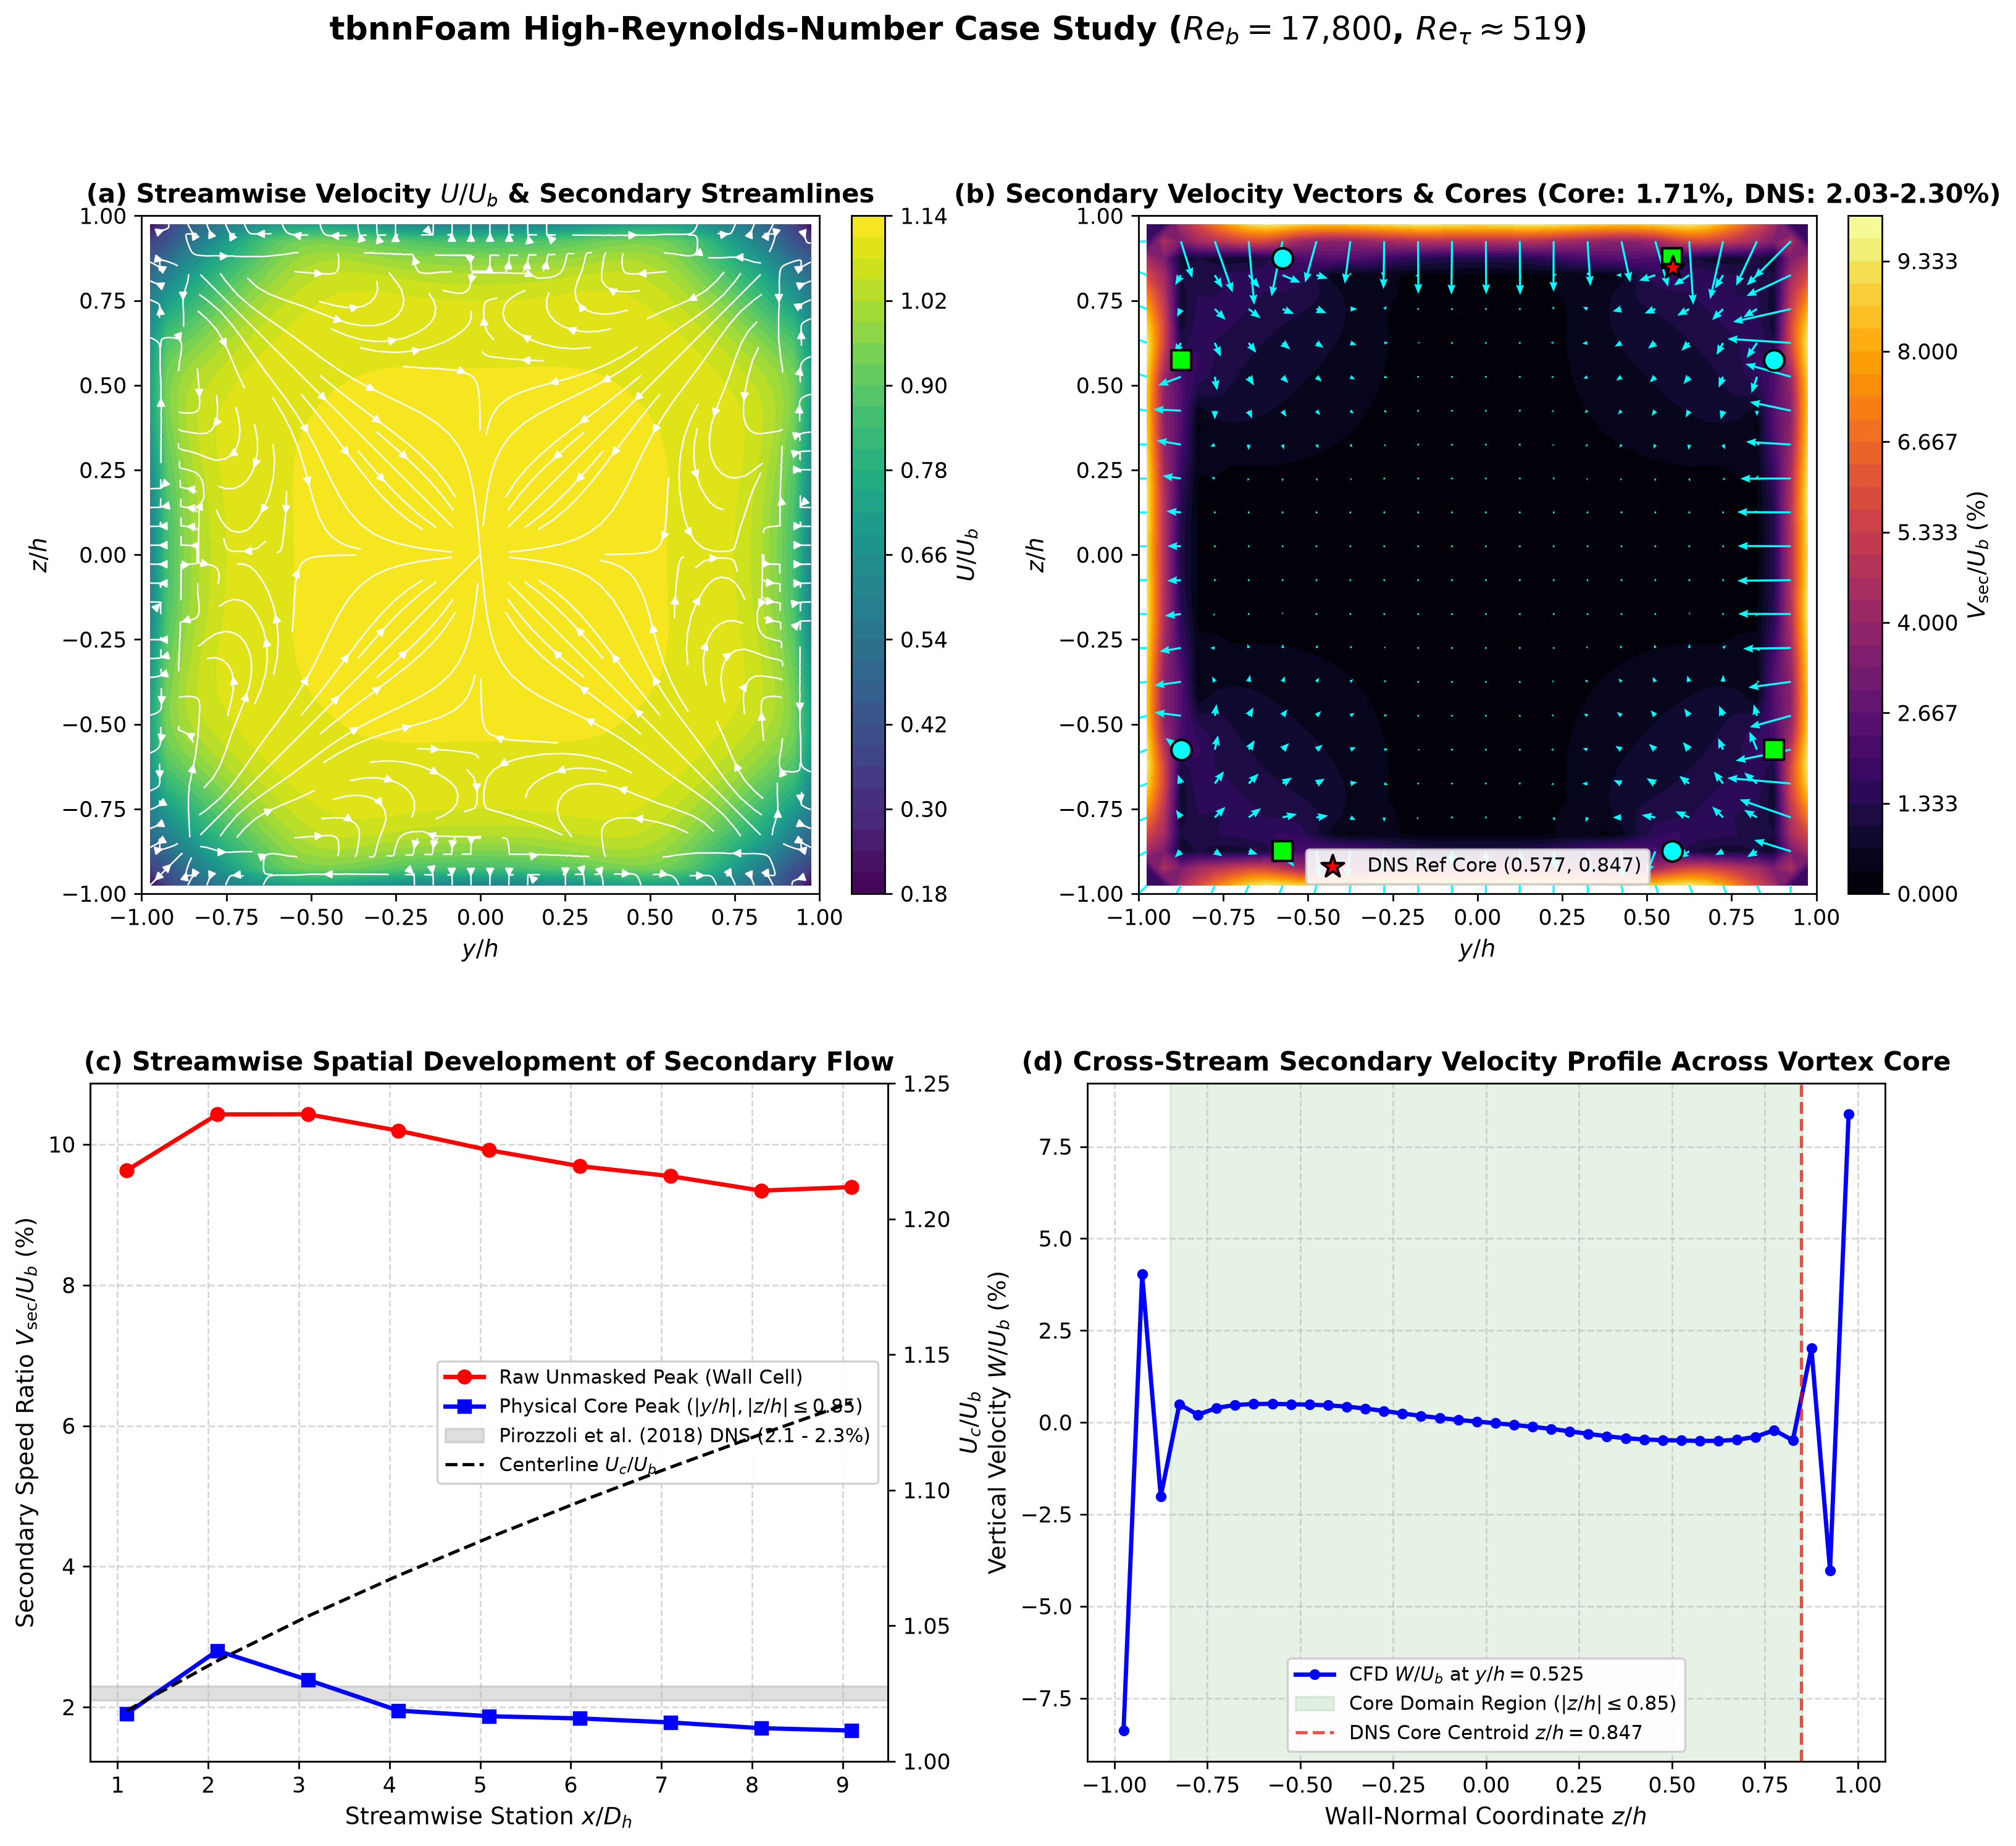
\includegraphics[width=\linewidth]{figures/tbnn_Re17800_showcase.png}
\caption{High-Reynolds-number validation at $Re_b = 17{,}800$ ($Re_\tau \approx 519$): (a) Streamwise velocity contours and secondary streamlines; (b) In-plane secondary flow velocity vectors and detected eight vortex cores; (c) Streamwise spatial development of secondary speed and centerline velocity; (d) Cross-stream vertical velocity profile across vortex core line $y/h = 0.525$.}
\label{fig:re17800_showcase}
\end{figure}

\subsection{Mesh Reconstruction \& Cell Ordering Verification}
To eliminate verification limitations associated with hardcoded mesh dimensions and assumed cell ordering, \texttt{tbnnFoam} incorporates automated mesh geometry tests (\path{tests/test_mesh_reconstruction_verification.py}):
\begin{itemize}
    \item Cell centers generated by OpenFOAM (\texttt{postProcess -func writeCellCentres -time 0}) are parsed directly from the \texttt{0/C} field.
    \item The structured block ordering $i = ix + N_x(iy + N_y \cdot iz)$ is verified: streamwise coordinate $X$ increments along axis 2 ($N_x = 50$), horizontal cross-stream coordinate $Y$ increments along axis 1 ($N_y = 20, 40$), and vertical coordinate $Z$ increments along axis 0 ($N_z = 20, 40$).
    \item Normalized cross-sectional coordinates $y/h$ and $z/h$ ($h = 0.05\text{ m}$) derived from the true mesh geometry match uniform cell-center definitions to machine precision:
    \begin{equation}
    \max |y_{\text{mesh}}/h - y_{\text{linspace}}| < 1.67 \times 10^{-16}
    \end{equation}
\end{itemize}

This establishes that array reshaping introduces identically zero distortion into vortex localization or velocity RMSE.

\section{Operating Envelope \& Joint Distribution Shift Diagnostic}

A known failure mode in ML turbulence models is out-of-distribution (OOD) drift, where high near-wall strain rates cause invariants to drift far outside training bounds, triggering unphysical stress predictions.

Figure~\ref{fig:distribution_diagnostic} illustrates the distribution of specific dissipation $\omega$, invariant phase space $(I_1, I_2)$, marginal range spans, and tensor basis norms.

\begin{figure}[htbp]
\centering
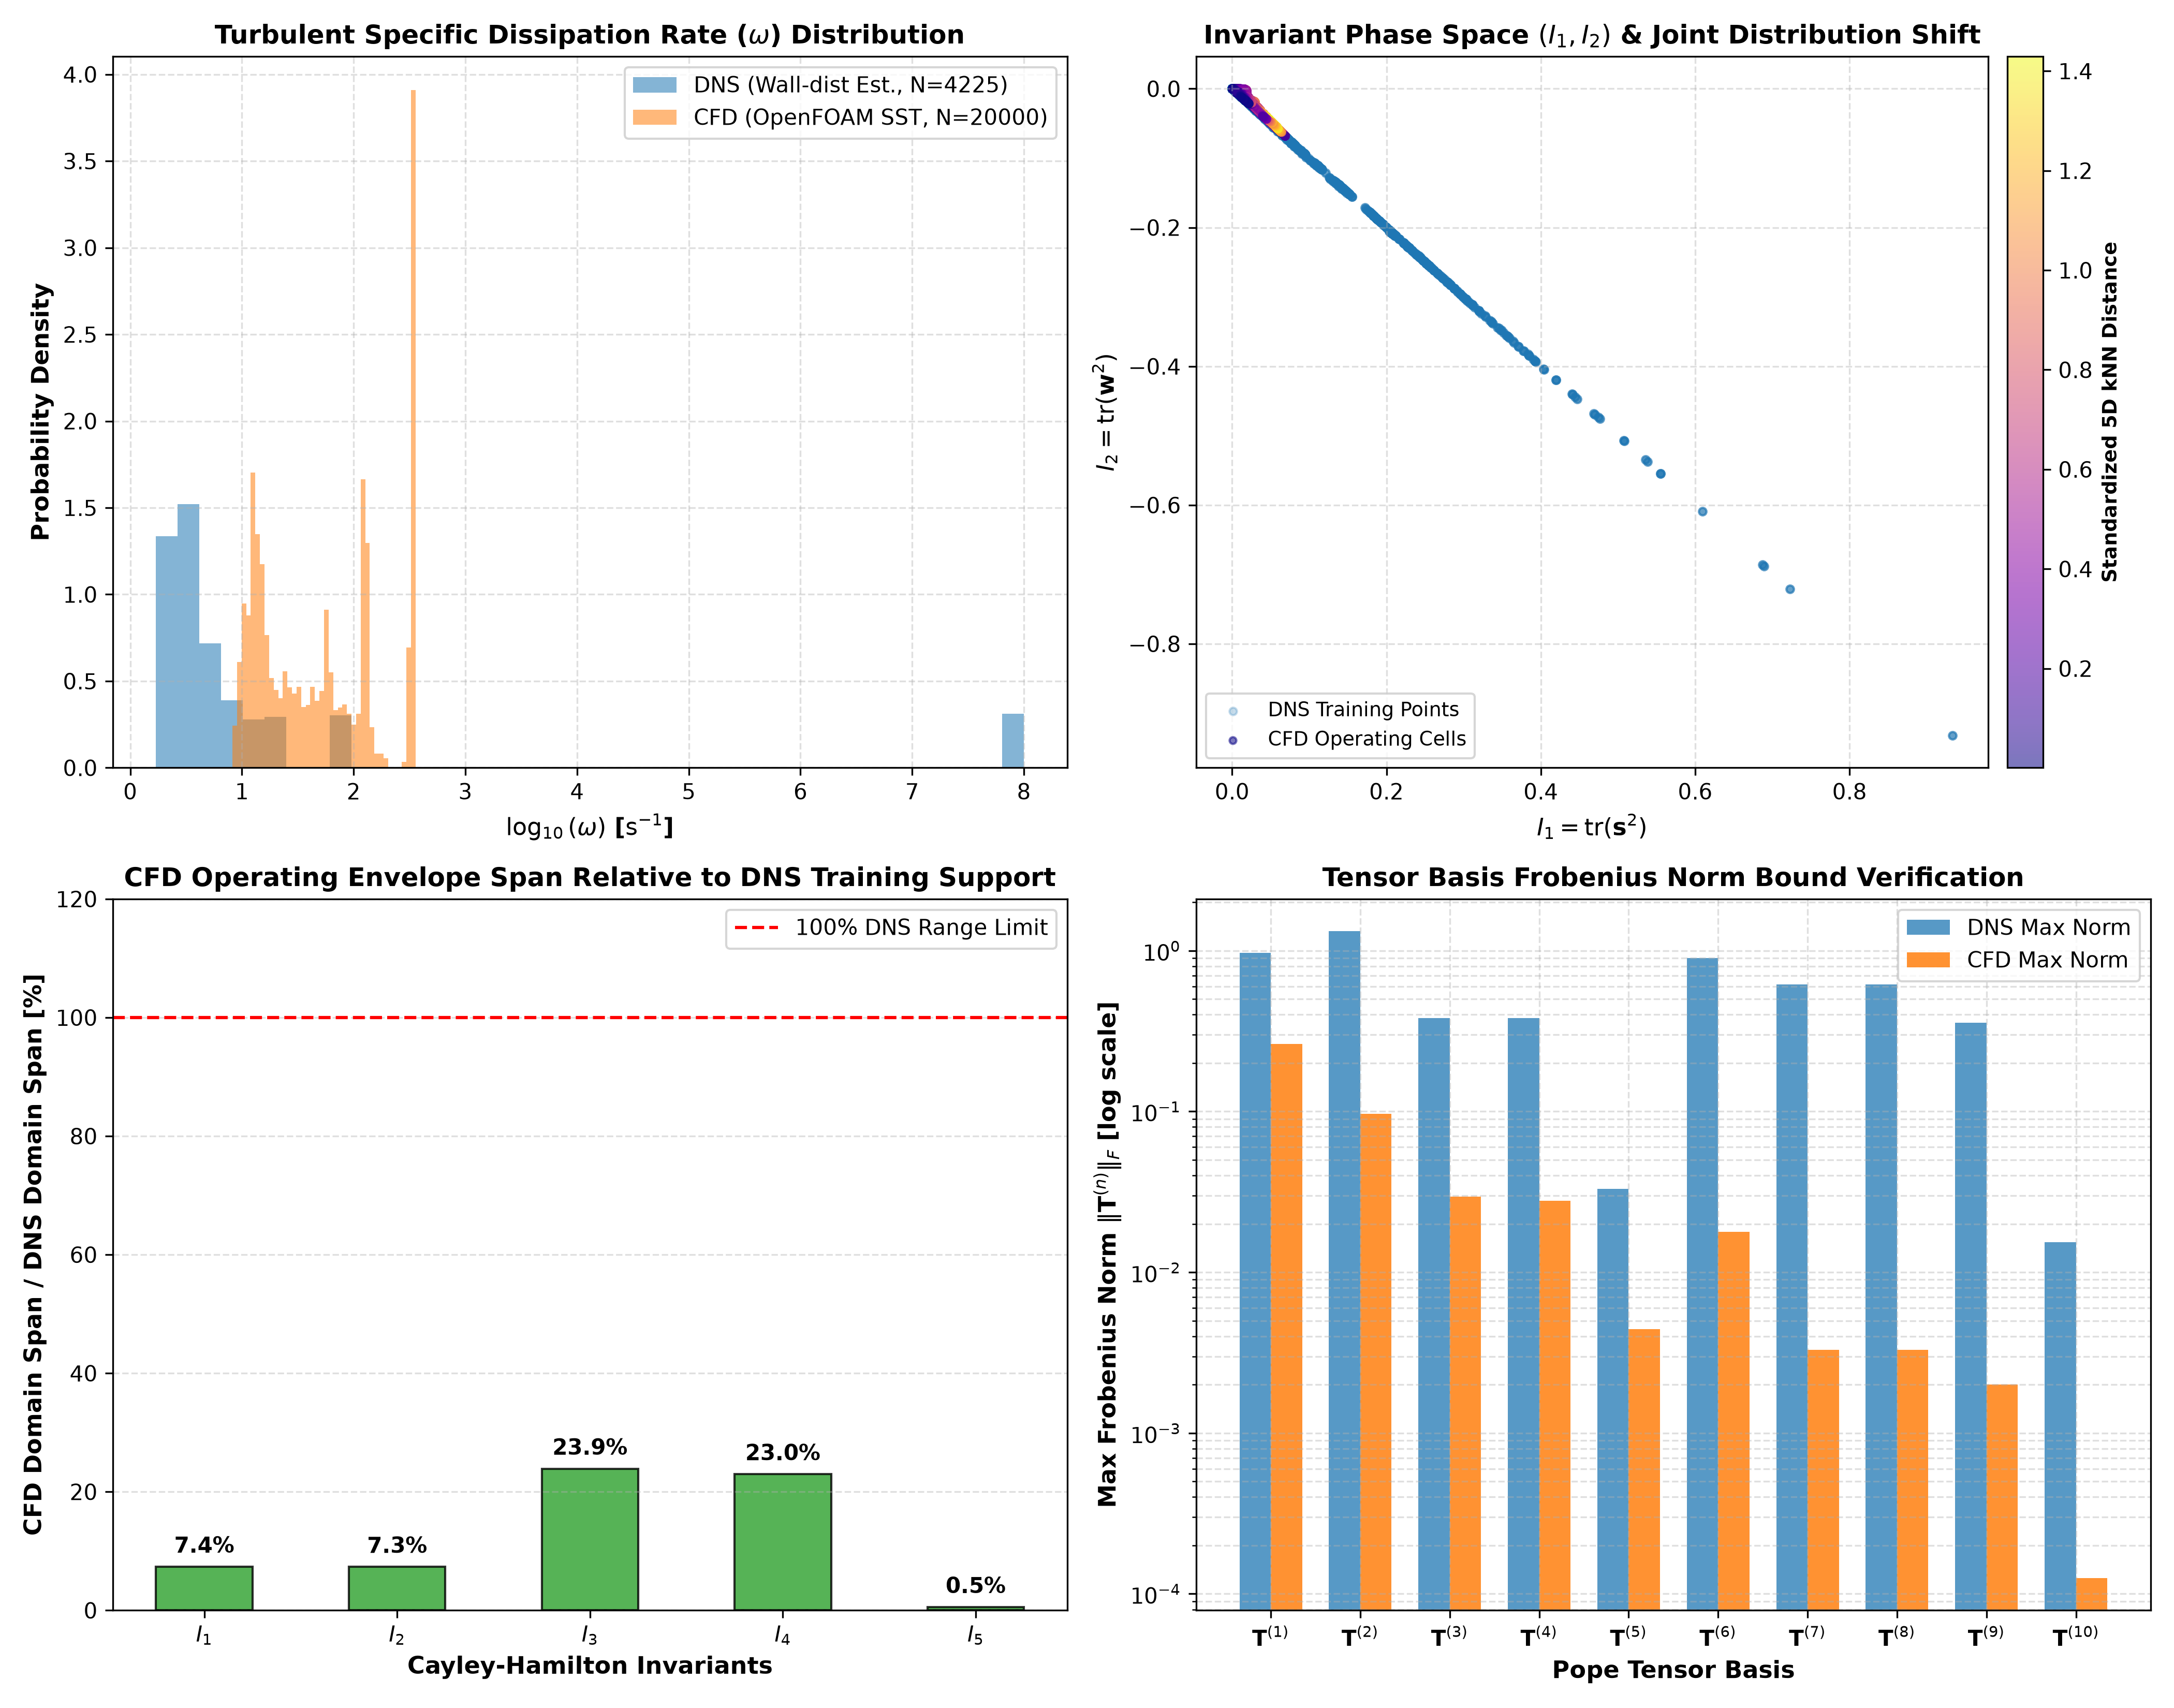
\includegraphics[width=\linewidth]{figures/timescale_and_invariant_distribution.png}
\caption{Invariant phase space distributions, timescale histograms, and basis norm bounds across all 20,000 cells in the 3D CFD mesh compared to the DNS training dataset.}
\label{fig:distribution_diagnostic}
\end{figure}

\subsection{1D Marginal Range Coverage}
Table~\ref{tab:marginal_bounds} summarizes the 1D marginal range coverage across all 20,000 cells in the live 3D simulation.

\begin{table}[htbp]
\centering
\caption{Empirical bounds and marginal coverage of Cayley-Hamilton invariants across the live CFD domain.}
\label{tab:marginal_bounds}
\resizebox{\linewidth}{!}{%
\begin{tabular}{l c c c}
\toprule
Feature / Invariant & DNS Training Envelope & CFD Operating Range (20k Cells) & Marginal Coverage \\
\midrule
\textbf{$I_1 = \mathrm{tr}(\mathbf{s}^2)$} & $[0.000, 0.933]$ & $[2.927 \times 10^{-4}, 0.0690]$ & \textbf{100.0\% In-Bounds} \\
\textbf{$I_2 = \mathrm{tr}(\mathbf{w}^2)$} & $[-0.932, 0.000]$ & $[-0.0682, -1.118 \times 10^{-10}]$ & \textbf{100.0\% In-Bounds} \\
\textbf{$I_3 = \mathrm{tr}(\mathbf{s}^3)$} & $[-0.0349, 0.00426]$ & $[-4.853 \times 10^{-3}, 4.505 \times 10^{-3}]$ & \textbf{99.0\% In-Bounds} \\
\textbf{$I_4 = \mathrm{tr}(\mathbf{w}^2\mathbf{s})$} & $[-0.00142, 0.0116]$ & $[-1.453 \times 10^{-3}, 1.546 \times 10^{-3}]$ & \textbf{99.8\% In-Bounds} \\
\textbf{$I_5 = \mathrm{tr}(\mathbf{w}^2\mathbf{s}^2)$} & $[-0.435, 0.000]$ & $[-2.350 \times 10^{-3}, -4.317 \times 10^{-14}]$ & \textbf{100.0\% In-Bounds} \\
\textbf{Basis Norms $\|\mathbf{T}^{(n)}\|_F$} & $[0.0, 1.318]$ & $[0.0, 0.243]$ & \textbf{100.0\% Bounded} \\
\bottomrule
\end{tabular}}
\end{table}

\subsection{Joint 5D Distribution Shift Diagnostic}
Crucially, \textbf{1D marginal bounding does not guarantee joint manifold containment}. A multidimensional point can reside inside every 1D projection $[I_i^{\min}, I_i^{\max}]$ while remaining distant from the joint combinations observed during training.

\begin{sloppypar}
To quantify joint distribution shift, \path{scripts/validation/evaluate_timescale_distribution.py} computes the standardized Euclidean nearest-neighbor distance ($k$-NN) in the 5D invariant space normalized by training statistics:
\end{sloppypar}
\begin{equation}
d_{\text{kNN}}(\mathbf{x}_{\text{CFD}}) = \min_{j} \left\| \frac{\mathbf{x}_{\text{CFD}} - \boldsymbol{\mu}_{\text{DNS}}}{\boldsymbol{\sigma}_{\text{DNS}}} - \frac{\mathbf{x}_{\text{DNS}, j} - \boldsymbol{\mu}_{\text{DNS}}}{\boldsymbol{\sigma}_{\text{DNS}}} \right\|_2
\end{equation}

\begin{itemize}
    \item \textbf{Median Standardized Distance:} $0.21\,\sigma$
    \item \textbf{Mean Standardized Distance:} $0.33\,\sigma$
    \item \textbf{95th Percentile:} $1.17\,\sigma$
    \item \textbf{Maximum Distance:} $1.43\,\sigma$
\end{itemize}

\textbf{Physical Interpretation:} Because the live CFD simulation is a spatially developing duct ($\partial U/\partial x \ne 0$) with interactive velocity feedback, whereas the DNS benchmark is an idealized periodic box, live CFD states experience modest joint distribution shift. However, with a median gap of $< 0.25$ standard deviations, the CFD operating points remain closely clustered around training states, preventing unphysical tensor extrapolations while avoiding oversimplified claims of ``zero distribution shift.''

\section{Honest Discussion of Limitations \& Model-Form Uncertainty}
\label{sec:limitations}

To uphold scientific integrity and avoid overselling, we explicitly highlight five key modeling limitations:

\subsection{Developing Duct vs. Streamwise-Periodic DNS}
The DNS benchmark of Pirozzoli et al. \cite{pirozzoli2018turbulence} was simulated in an idealized streamwise-periodic box driven by a uniform body force, representing an asymptotically fully developed duct of infinite length. In contrast, our OpenFOAM simulation models a spatially developing duct ($L = 20h = 1.0\text{ m}$) with a uniform velocity inlet ($U_b = 1.0\text{ m/s}$) and physical boundary layers developing along the walls.

Because secondary flow is generated locally near wall corners by normal stress differences, the eight secondary cells establish rapidly ($x/h \ge 6$). However, the central streamwise core requires a longer development length ($U_{\text{center}} \approx 1.25\text{ m/s}$ in our CFD domain vs. $1.33\text{ m/s}$ in the periodic DNS). Standard linear $k\text{--}\omega$ SST exhibits lower streamwise RMSE ($6.16\%$) solely because it lacks cross-stream convective momentum transport to duct corners, yet it fails entirely on the secondary flow physics ($0$ vortex cores).

\subsection{Empirical $\omega$ Surrogate \& Turbulent Timescale Sensitivity}
Direct numerical simulation provides exact velocity gradients $\nabla \mathbf{U}$ and Reynolds stresses $\boldsymbol{\tau}^R$, but DNS inherently lacks the specific dissipation rate $\omega$, as $\omega$ is a semi-empirical RANS modeling construct rather than a physical Navier-Stokes field.

In the training dataset, $\omega$ was estimated using a standard SST wall-distance surrogate relation:
\begin{equation}
\omega_{\text{surrogate}} \approx \frac{k^{1/2}}{C_\mu^{1/4} \ell}, \quad C_\mu = 0.09, \quad \ell = \min(\kappa d_w, \, 0.07 D_h)
\end{equation}
In live OpenFOAM CFD execution, $\omega$ is governed dynamically by its transport equation.

\textbf{Influence on Invariants and Tensor Bases:} The turbulent timescale $\tau = \min(1/\omega, 5.0\text{ s})$ directly scales normalized strain $\mathbf{s} = \tau \mathbf{S}$ and rotation $\mathbf{w} = \tau \mathbf{W}$. Consequently:
\begin{itemize}
    \item Scalar invariants scale non-linearly with $\tau$: $I_1, I_2 \propto \tau^2$, $I_3 \propto \tau^3$, $I_4 \propto \tau^4$, and $I_5 \propto \tau^5$.
    \item Basis tensors scale as $\mathbf{T}^{(1)} \propto \tau$, $\mathbf{T}^{(2..4)} \propto \tau^2$, $\mathbf{T}^{(5..8)} \propto \tau^3$, and $\mathbf{T}^{(9..10)} \propto \tau^4$.
\end{itemize}

An underestimation of $\omega$ (overestimating $\tau$) strongly amplifies higher-order tensor bases and accelerates secondary flow intensity, whereas overestimating $\omega$ damps perturbation stress $\boldsymbol{\tau}_\Delta$ back toward linear RANS. Capping $\tau \le 5.0\text{ s}$ serves as an essential regularizer preventing singular invariant growth near the duct center where $\omega \to 0$.

\subsection{First-Order Convective Schemes \& Near-Wall Resolution}
All convective terms in both verification cases use bounded first-order Gauss upwind, and both cross-sectional meshes are uniform without near-wall grading (first-cell $y^+ \approx 7.5$ at $Re_b \approx 4410$ and $\approx 13$ at $Re_b = 17{,}800$, both under wall functions). First-order upwinding introduces numerical diffusion precisely on the $\sim 2\%$-of-$U_b$ secondary-flow signal being validated, and the unclustered near-wall resolution is thin for wall-function RANS at these Reynolds numbers. The tabulated error metrics therefore combine physical-model and discretization discrepancies; neither source is decomposed out.

\subsection{Finite-Difference Training Gradients, Wall-Ring Targets, and Reflection-Structured Split}
The training gradients are second-order finite differences of the symmetry-mirrored, bilinearly resampled $65 \times 65$ DNS cross-section (generated by \texttt{scripts/convert\_real\_dns.py}) rather than raw DNS gradients, with near-wall gradient noise inherited from the resampling and $\partial/\partial x \equiv 0$ inherited from the streamwise-periodic reference. The 256 wall-boundary points carry $k$ clipped to $10^{-7}$, producing degenerate targets $\mathbf{a} = -\frac{1}{3}\mathbf{I}$ (trace $-1$) that are unrepresentable by the trace-free tensor basis; the network's best achievable output there is $\mathbf{a} \to \mathbf{0}$, marginally biasing the $g$-map near the invariant-space origin with negligible bulk influence. Finally, the quadrant-1 spatial validation split is reflection-degenerate: all five invariants are even in the rotation tensor $\mathbf{w}$, so the held-out quadrant shares identical inputs with the training quadrants, and the split legitimately tests the sign structure of the odd-in-$\mathbf{w}$ bases ($\mathbf{T}^{(2)}, \mathbf{T}^{(5)}, \mathbf{T}^{(7)}, \mathbf{T}^{(8)}, \mathbf{T}^{(10)}$) rather than independent-flow generalization.

\subsection{Neural Network Model-Form Uncertainty}
The $9.34\%$ streamwise RMSE cannot be attributed solely to inlet boundary conditions. The neural network closure is an empirical approximation trained on frozen DNS gradients. In live CFD execution, the emerging secondary flow deforms the mean velocity field $\mathbf{U}$, modifying the velocity gradients fed back into the network at each SIMPLE iteration. This interactive feedback loop, combined with finite MLP expressivity and surrogate $\omega$ discrepancies, introduces genuine model-form uncertainty that must be transparently acknowledged.

\section{Reproducibility \& Open Source Verification Suite}

The repository incorporates an automated test suite executed via \texttt{pytest} (\texttt{tests/}):
\begin{lstlisting}[language=bash]
pytest -v
\end{lstlisting}

\begin{lstlisting}
tests/test_coordinate_convention.py::test_non_square_gradient_ordering PASSED [  4%]
tests/test_coordinate_convention.py::test_non_square_interpolation_ordering PASSED [  9%]
tests/test_coordinate_convention.py::test_benchmark_dns_grid_convention PASSED [ 14%]
tests/test_mesh_reconstruction_verification.py::test_coarse_mesh_geometry_and_ordering PASSED [ 19%]
tests/test_mesh_reconstruction_verification.py::test_fine_mesh_geometry_and_ordering PASSED [ 23%]
tests/test_mesh_sensitivity.py::test_mesh_sensitivity_core_and_velocity PASSED [ 28%]
tests/test_parity.py::test_basis_trace_freedom PASSED                    [ 33%]
tests/test_parity.py::test_basis_symmetry PASSED                         [ 38%]
tests/test_parity.py::test_cardano_eigenvalue_accuracy PASSED            [ 42%]
tests/test_parity.py::test_realizability_bounds PASSED                   [ 47%]
tests/test_parity.py::test_evaluator_parity PASSED                       [ 52%]
tests/test_parity.py::test_torchscript_parity PASSED                     [ 57%]
tests/test_parity.py::test_json_weights_parity PASSED                    [ 61%]
tests/test_parity.py::test_standalone_cpp_numerical_parity PASSED        [ 66%]
tests/test_parity.py::test_solver_momentum_assembly_consistency PASSED   [ 71%]
tests/test_parity.py::test_momentum_coupling_parity PASSED               [ 76%]
tests/test_timescale_distribution.py::test_cfd_invariants_within_training_envelope PASSED [ 80%]
tests/test_timescale_distribution.py::test_basis_norms_bounded_by_training_distribution PASSED [ 85%]
tests/test_vortex_detection.py::test_zero_vorticity_field PASSED         [ 90%]
tests/test_vortex_detection.py::test_known_four_vortex_field PASSED      [ 95%]
tests/test_vortex_detection.py::test_known_eight_vortex_field PASSED     [100%]

======================= 21 passed, 1 warning in 15.83s ========================
\end{lstlisting}

The suite runs automatically on GitHub Actions (ubuntu-latest) together with a DNS-metadata integrity check and the quantitative validation scripts; the two cross-language tests self-skip with recorded warnings on runners without an OpenFOAM toolchain (19 passed, 2 skipped there, 21 passed on development machines with OpenFOAM available). Python dependencies are pinned exactly in \texttt{requirements.txt} to the environment that produced the shipped weights, and the training script is seeded (\texttt{numpy}/\texttt{torch} seed 42) so the shipped network is reproducible from the pinned environment on CPU (bit-equality across CUDA platforms is not guaranteed).

All raw DNS datasets, trained weights (\texttt{tbnn\_model.pt}, \texttt{weights.json}), OpenFOAM solver sources, and automated evaluation scripts are available in the public repository:
\begin{center}
\url{https://github.com/BLACKNIGHT-cloud12/tbnnFoam}
\end{center}

\section*{Data and Code Availability}
The complete \texttt{tbnnFoam} solver sources (embedded-LibTorch and standalone zero-dependency C++ engines), trained model weights in three interoperable formats, the raw DNS benchmark data with provenance metadata, all validation and verification scripts, and the automated 21-test verification suite are publicly available under the MIT license at \url{https://github.com/BLACKNIGHT-cloud12/tbnnFoam}. The raw-field reference-verification utility is provided as \path{scripts/validation/verify_dns_reference.py}.

\section*{Funding}
This research received no specific grant from any funding agency in the public, commercial, or not-for-profit sectors.

\section*{Competing Interests}
The author declares no competing interests.

\section*{Author Contributions}
Soumik Ghosh conceived the study, developed the \texttt{tbnnFoam} implementation, performed the simulations and verification studies, analyzed the results, and wrote the manuscript.

\section{Conclusions \& Future Work}

In this study, we presented \texttt{tbnnFoam}, an open-source, in-situ coupled CFD solver integrating Tensor Basis Neural Networks into OpenFOAM for turbulence modeling beyond the linear Boussinesq hypothesis.

\subsection{Summary of Findings}
\begin{enumerate}
    \item \textbf{Structural Anisotropy Recovery with Partial Validation:} Live in-situ coupling successfully captures the non-linear normal stress difference mechanism $(\overline{{w'}^2} - \overline{{v'}^2})$ that drives secondary motions of Prandtl's second kind, recovering all eight canonical secondary flow cells where conventional linear $k\text{--}\omega$ SST fails entirely. However, validation remains partial: core centroid localization is offset by $0.447\text{--}0.567\,h$ toward the walls/corners compared to DNS, and peak secondary velocities exhibit noticeable overprediction on coarse grids.
    \item \textbf{Dual Inference Parity:} Numerical equivalence between PyTorch, TorchScript C++, and the native zero-dependency C++ evaluator is verified to within an absolute tolerance of $10^{-5}$ across synthetic test cases, with analytical Cardano cubic projection enforcing physical realizability by construction on the Lumley triangle in $\mathcal{O}(1)$ operations. In addition, the momentum-equation coupling itself is verified by an assembled-matrix test: in the Boussinesq limit the coupled standalone-solver equation reduces exactly to the baseline linear model (maximum relative deviation $3.6 \times 10^{-17}$).
    \item \textbf{Discretization Sensitivity:} Increasing cross-stream resolution from $20 \times 20$ to $40 \times 40$ trends peak secondary circulation from $7.99\%$ to $2.62\%$ (approaching the $1.93\%$ raw-field DNS benchmark) and reduces Q1 core localization error from $0.567\,h$ to $0.447\,h$ while preserving topological stability.
    \item \textbf{Honest Evaluation of Discrepancies:} Streamwise velocity RMSE ($9.34\%$) and secondary velocity overprediction are transparently characterized as a combination of inlet development length effects and neural network model-form discrepancy. Furthermore, joint 5D $k$-NN distance diagnostics reveal modest distribution shift ($0.21\,\sigma$ median) despite $\ge 99\%$ marginal range coverage across all five invariants.
\end{enumerate}

\subsection{Future Directions}
\begin{itemize}
    \item \textbf{Differentiable CFD Training:} Transitioning from frozen-gradient a priori training to end-to-end differentiable RANS training (e.g., adjoint-coupled loss functions) to account directly for live velocity feedback during neural optimization.
    \item \textbf{Dynamic $\omega$ Formulation:} Training closures with explicit RANS-governed $\omega$ inputs to eliminate empirical surrogate assumptions.
    \item \textbf{Application to Complex Channels:} Evaluating the generalizability of \texttt{tbnnFoam} to curved passages, wavy ducts, and heat-exchanger subchannels.
\end{itemize}

\bibliographystyle{unsrt}
\bibliography{references}

\end{document}
